\documentclass{article}
\usepackage{graphicx}
\usepackage{float}
\usepackage{geometry}
\usepackage{amsmath}
\usepackage{amssymb}
\geometry{a4paper, margin=1in}

\title{Task 6: Automated Parameter Tuning}
\author{Open Group 3}

\begin{document}

\maketitle 
\section{Introduction}
In this task, we aim to optimize the \texttt{LMR\_slope} (Late Move Reduction slope) parameter of the \texttt{SchachMaus} engine. We fix the other engine parameters to the recommended reasonable values: \texttt{NMP\_intercept} $= 3$, \texttt{NMP\_slope} $= 0$, \texttt{LMR\_intercept} $= 1$, \texttt{RFP\_intercept} $= -30$, \texttt{RFP\_slope} $= 150$.
\par We seek to optimize \texttt{LMR\_slope} over the interval $[0, 2]$ for a time control of $30$ seconds$+0$. In the language of Lecture 8, we are optimizing the function:
\[
f: [0,2] \to \mathbb{R}, \quad f(x) = \text{Elo rating of engine with (LMR\_slope} = x\text{)}
\]
We approximate the function $f$ by playing games between engines with varying $x$-parameters and using Task 1 to estimate the ratings (relative to one another). This yields evaluation data with noisy measurements, where the noise $\epsilon$ corresponds to the standard deviation of the posterior rating distribution obtained from Task 1.

\section{Initialization and Initial Data Collection}
We began by defining a range of initial \texttt{LMR\_slope} values $\{0, 0.5, 1.0, 1.5, 2.0\}$. Five engine instances were initialized with these parameters and played a round-robin tournament. Each pair played 50 games (25 random positions $\times$ 2 colors) to establish a baseline rating.

These were the results:
\begin{figure}[H]
    \centering
    % Ensure this file exists in your directory or remove this block
    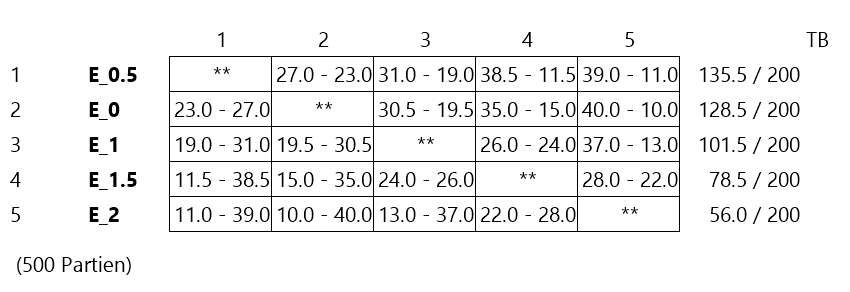
\includegraphics[width=0.7\textwidth]{tournament_table_after_initial_tournament.png}
    \caption{Tournament table after the initial round-robin phase.}
    \label{fig:init_table}
\end{figure}

\paragraph{Intuition for LMR Slope:}
Late Move Reduction (LMR) is a search heuristic used to reduce the depth of searches for moves that are assumed to be bad. The \texttt{LMR\_slope} parameter probably controls how aggressively this reduction scales with the move index and depth. A value of $0$ implies searching everything more deeply, compared to a higher value like $2.0$. Higher values risk missing good moves, but save time that can be used for other calculations.

\par From the initial results, we observed that engines with lower slopes performed significantly better than those with higher slopes.  Here is an example from the tournament, that illustrates the difference quite well:
\par The white engine was initialized with parameter LMR\_slope = 0, and black had LMR\_slope = 2.
\begin{figure}[H]
    \centering
    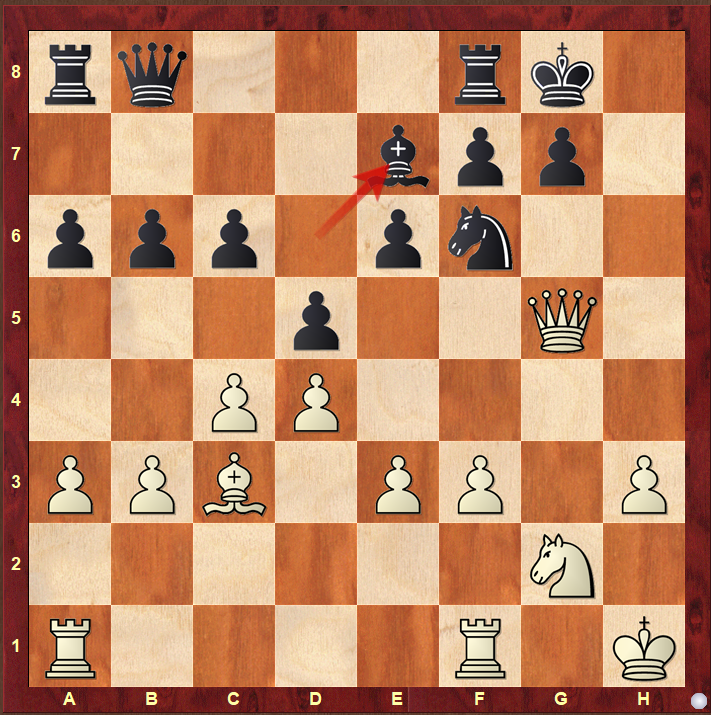
\includegraphics[width=0.6\textwidth]{game54_be7.png}
    \caption{Position after \textbf{25. ... Be7?}}
    \label{fig:pos1}
\end{figure}

\noindent \textbf{Continuation:} \\
26. Nf4 dxc4 27. Rg1 g6

\begin{figure}[H]
    \centering
    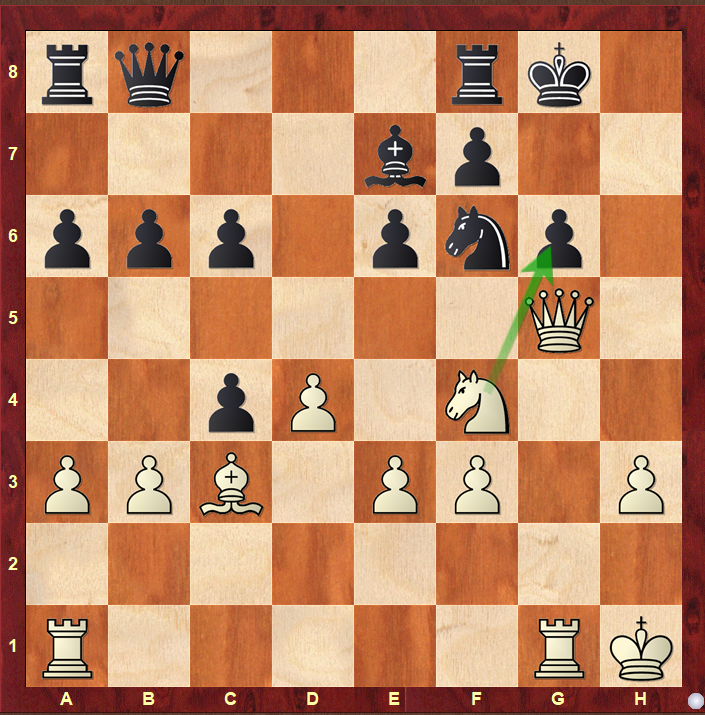
\includegraphics[width=0.6\textwidth]{game54_Nxg6.png}
    \caption{Position before \textbf{28. Nxg6}}
    \label{fig:pos2}
\end{figure}
and White won.\par We need to find the "sweet spot" between reducing the LMR to accellerate calculation, but not too much so as not to risk missing important resources. From the initial tournament result, it seems likely that the optimal LMR\_slope-parameters, are rather in the first half of $[0,2]$.
\par Turning toward the analysis:\newline We used the Stan model from Task 1 to estimate $f$ at the initial values:
\begin{figure}[H]
\begin{verbatim}
D <- run_elo_model("tournament_results.csv", stanmodel)
\end{verbatim}
\end{figure}

We then calculated the Gaussian Process (GP) as a surrogate model for $f$. The \texttt{DiceKriging} package provides built-in functionality to model a Gaussian Process with a Gaussian kernel and known noise variances:

\begin{figure}[H]
\begin{verbatim}
library(DiceKriging)
kernel_type <- "gauss"

# Fit the GP
gp_model <- km(
  design = data.frame(x = as.numeric(sub("E_", "", D$X))), 
  response = D$Y, 
  covtype = kernel_type, 
  noise.var = D$epsilon^2,
  upper = 0.3 # upper bound for length-scale parameter
)
\end{verbatim}
\caption{Fitting the Gaussian Process.}
\end{figure}

\paragraph{Heuristic for length-scale constraint:}
Our initial data points are spaced by $0.5$. A length-scale of $0.3$ makes the uncertainty (confidence intervals) grow in the gaps between the points, with "peak uncertainty" around $0.2$ to $0.3$, $0.7$ to $0.8$ and so on. This prevents the model from starting the search close to the initial maximum $0.5$ immediately, and makes it explore the gaps a bit first.

\par For the acquisition function, we calculate the Expected Improvement (EI) using the formula from Lecture 8:

\begin{figure}[H]
\begin{verbatim}
calculate_expected_improvement <- function(pred, y_best){
  # pred = prediction of GP model for some points X
  # returns expected improvement for points X
  
  mu <- pred$mean
  sigma <- pred$sd
  sigma <- pmax(sigma, 1e-9) # avoid division by zero

  # Calculate Expected Improvement
  Z <- (mu - y_best) / sigma
  # Formula: (mu - y_best) * Phi(Z) + sigma * phi(Z)
  ei <- (mu - y_best) * pnorm(Z) + sigma * dnorm(Z)
  
  return(ei)
}
\end{verbatim}
\caption{Expected Improvement Implementation.}
\end{figure}

\paragraph{Initial Plot:}
The plot below visualizes the state of the optimization before the loop begins. The blue line represents the GP mean prediction, and the shaded area is the $95\%$ confidence interval. The red line shows the Expected Improvement (scaled for visualization), indicating where the model suggests we should sample next to potentially find a better parameter.

\begin{figure}[H]
    \centering
    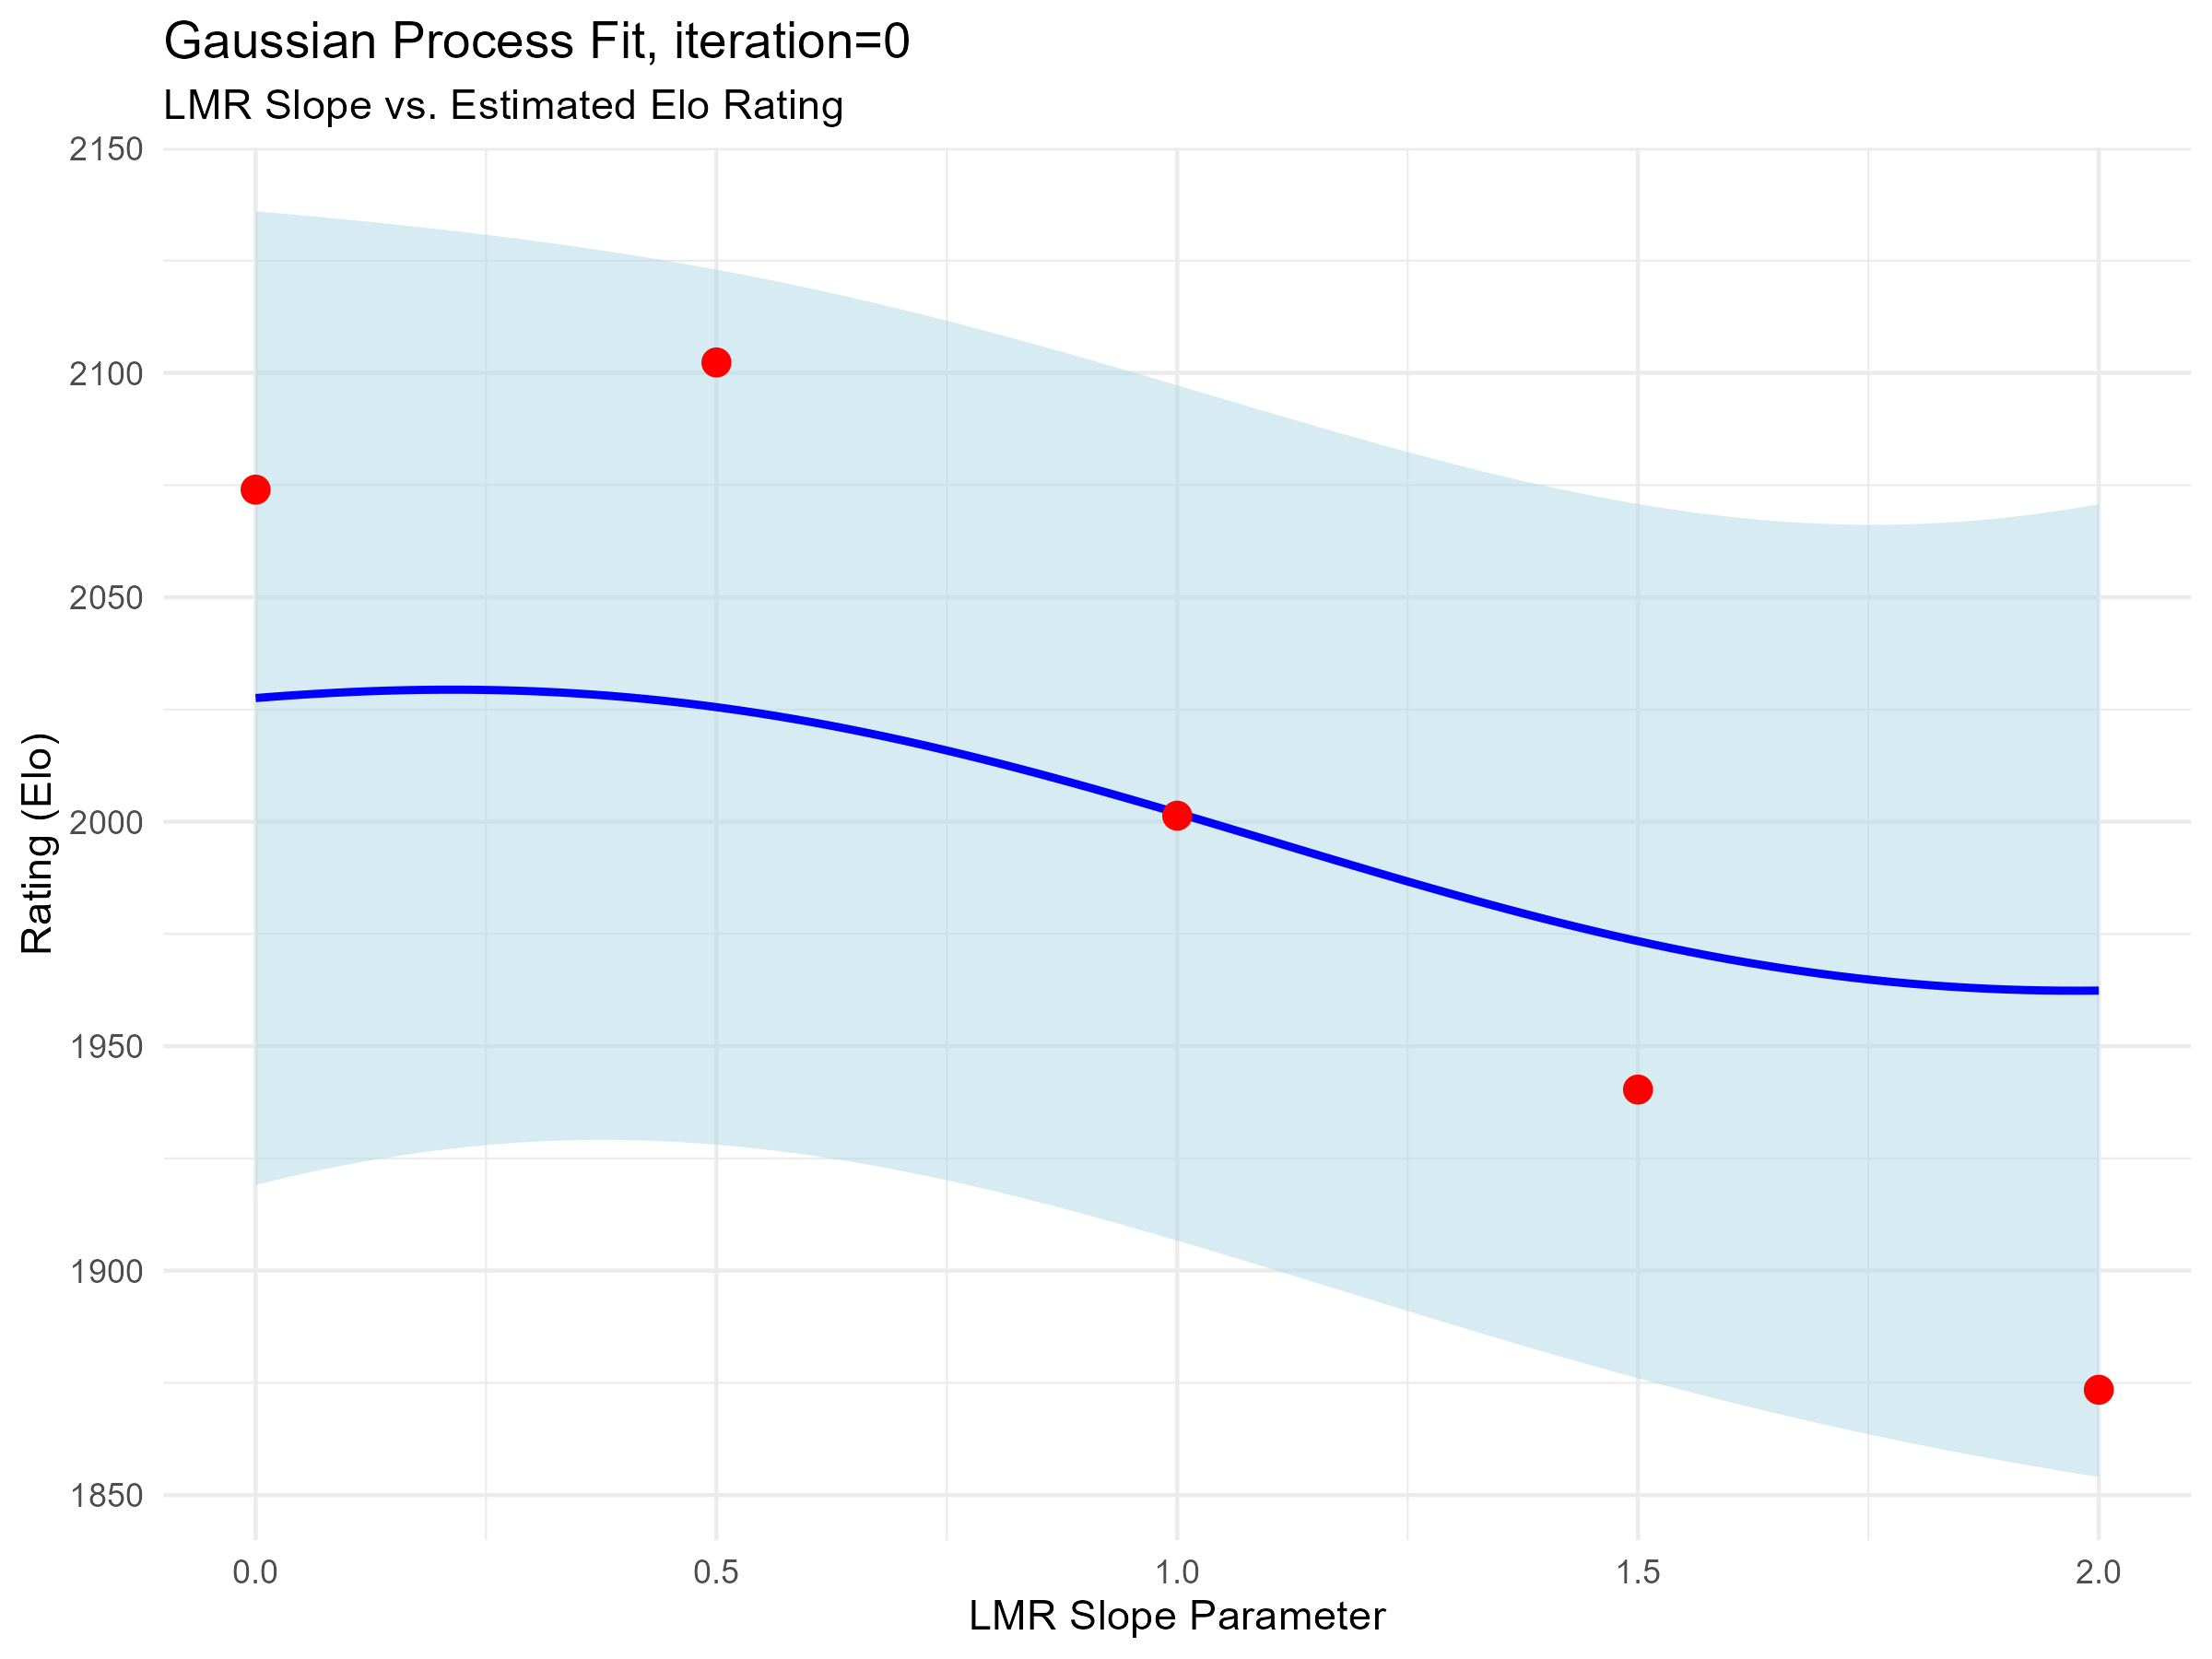
\includegraphics[width=0.8\textwidth]{initial_plot.png}
    \caption{Initial GP fit (Iteration 0) based on the 5 starting engines.}
    \label{fig:iter0}
\end{figure}

\section{Optimization Loop}
In each iteration, we maximize the expected improvement function to identify the next candidate parameter. We also calculate the probability of improvement.

\par The new candidate engine plays a mini-tournament against a diverse subset of existing engines: the current \textbf{Best}, \textbf{2nd Best}, \textbf{Median}, and \textbf{Worst} engines. A weighted round schedule (15, 10, 5, 2 games respectively) was used to prioritize accurate comparisons against the top engines. The weaker engines (Median/Worst) are included as further reference to the rating pool.

\par The new games are appended to the PGN file. We then re-run the rating model from Task 1 on all games to update the rating estimates for all engines, including the new one. Finally, we update the GP model with the new data point and plot the result.

The optimization process is visualized below:

\begin{figure}[H]
    \centering
    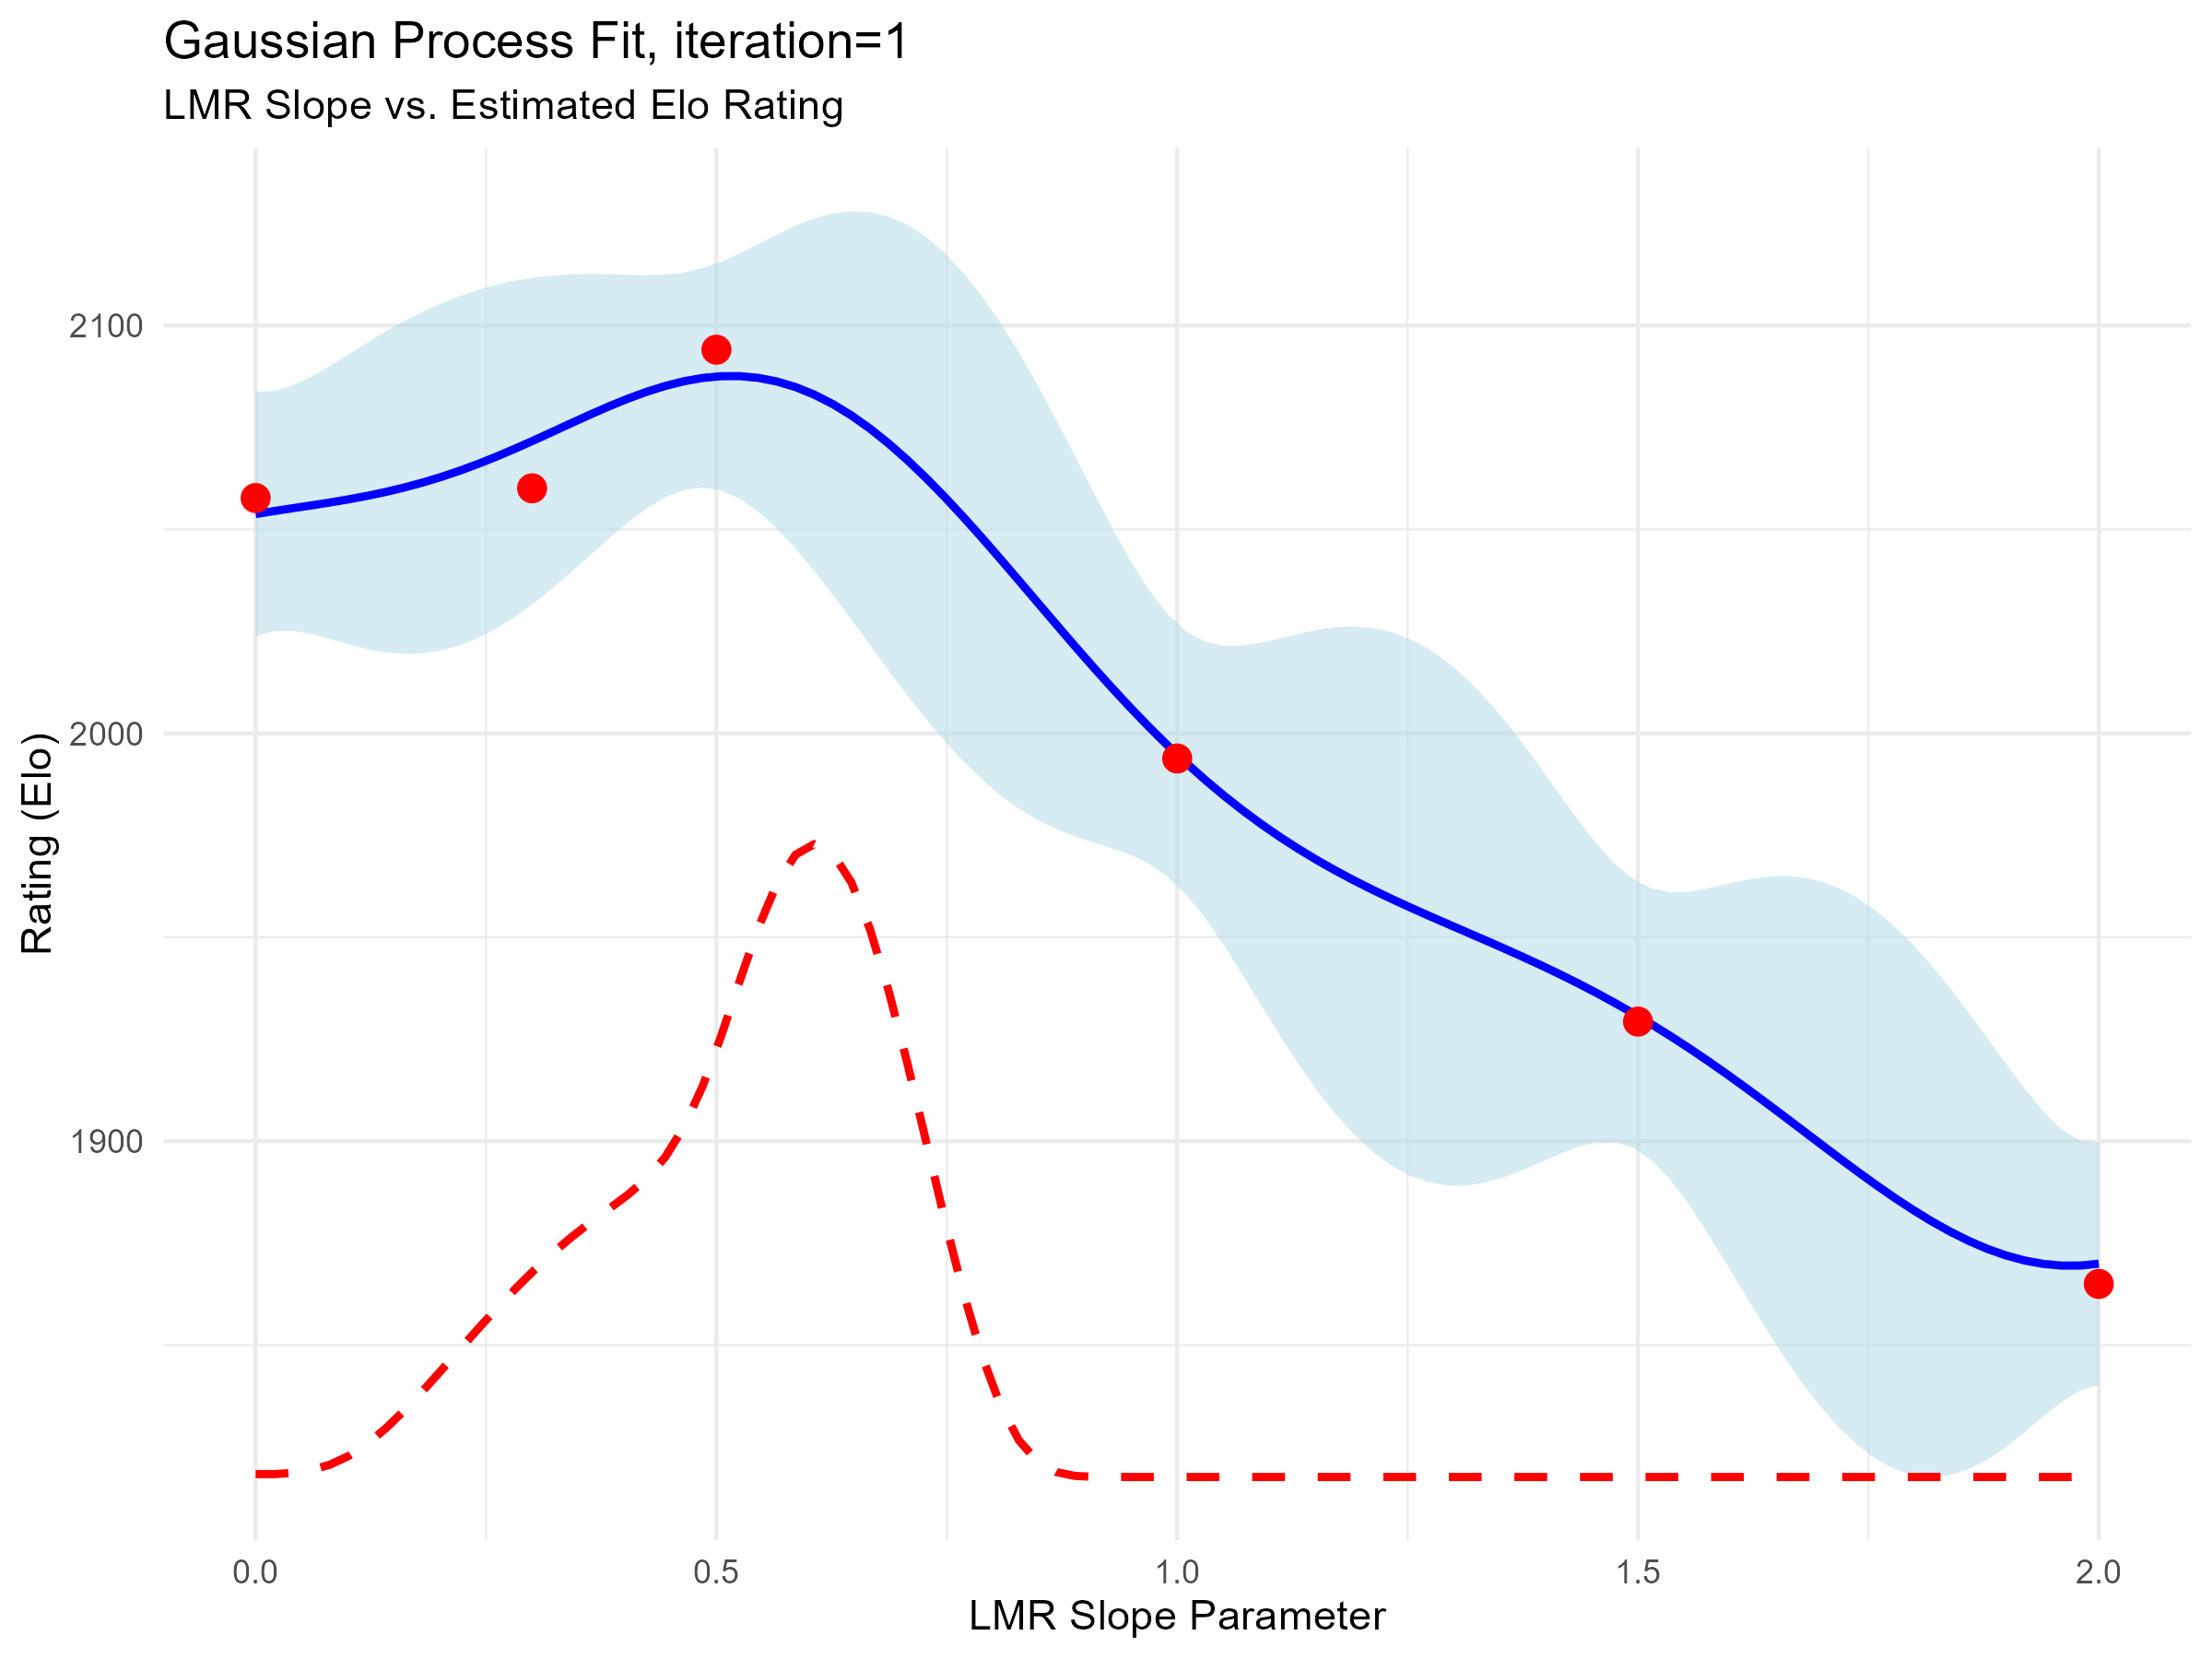
\includegraphics[width=0.8\textwidth]{optimization_iteration_1.png}
    \caption{GP fit after Iteration 1.}
    \label{fig:iter1}
\end{figure}

\begin{figure}[H]
    \centering
    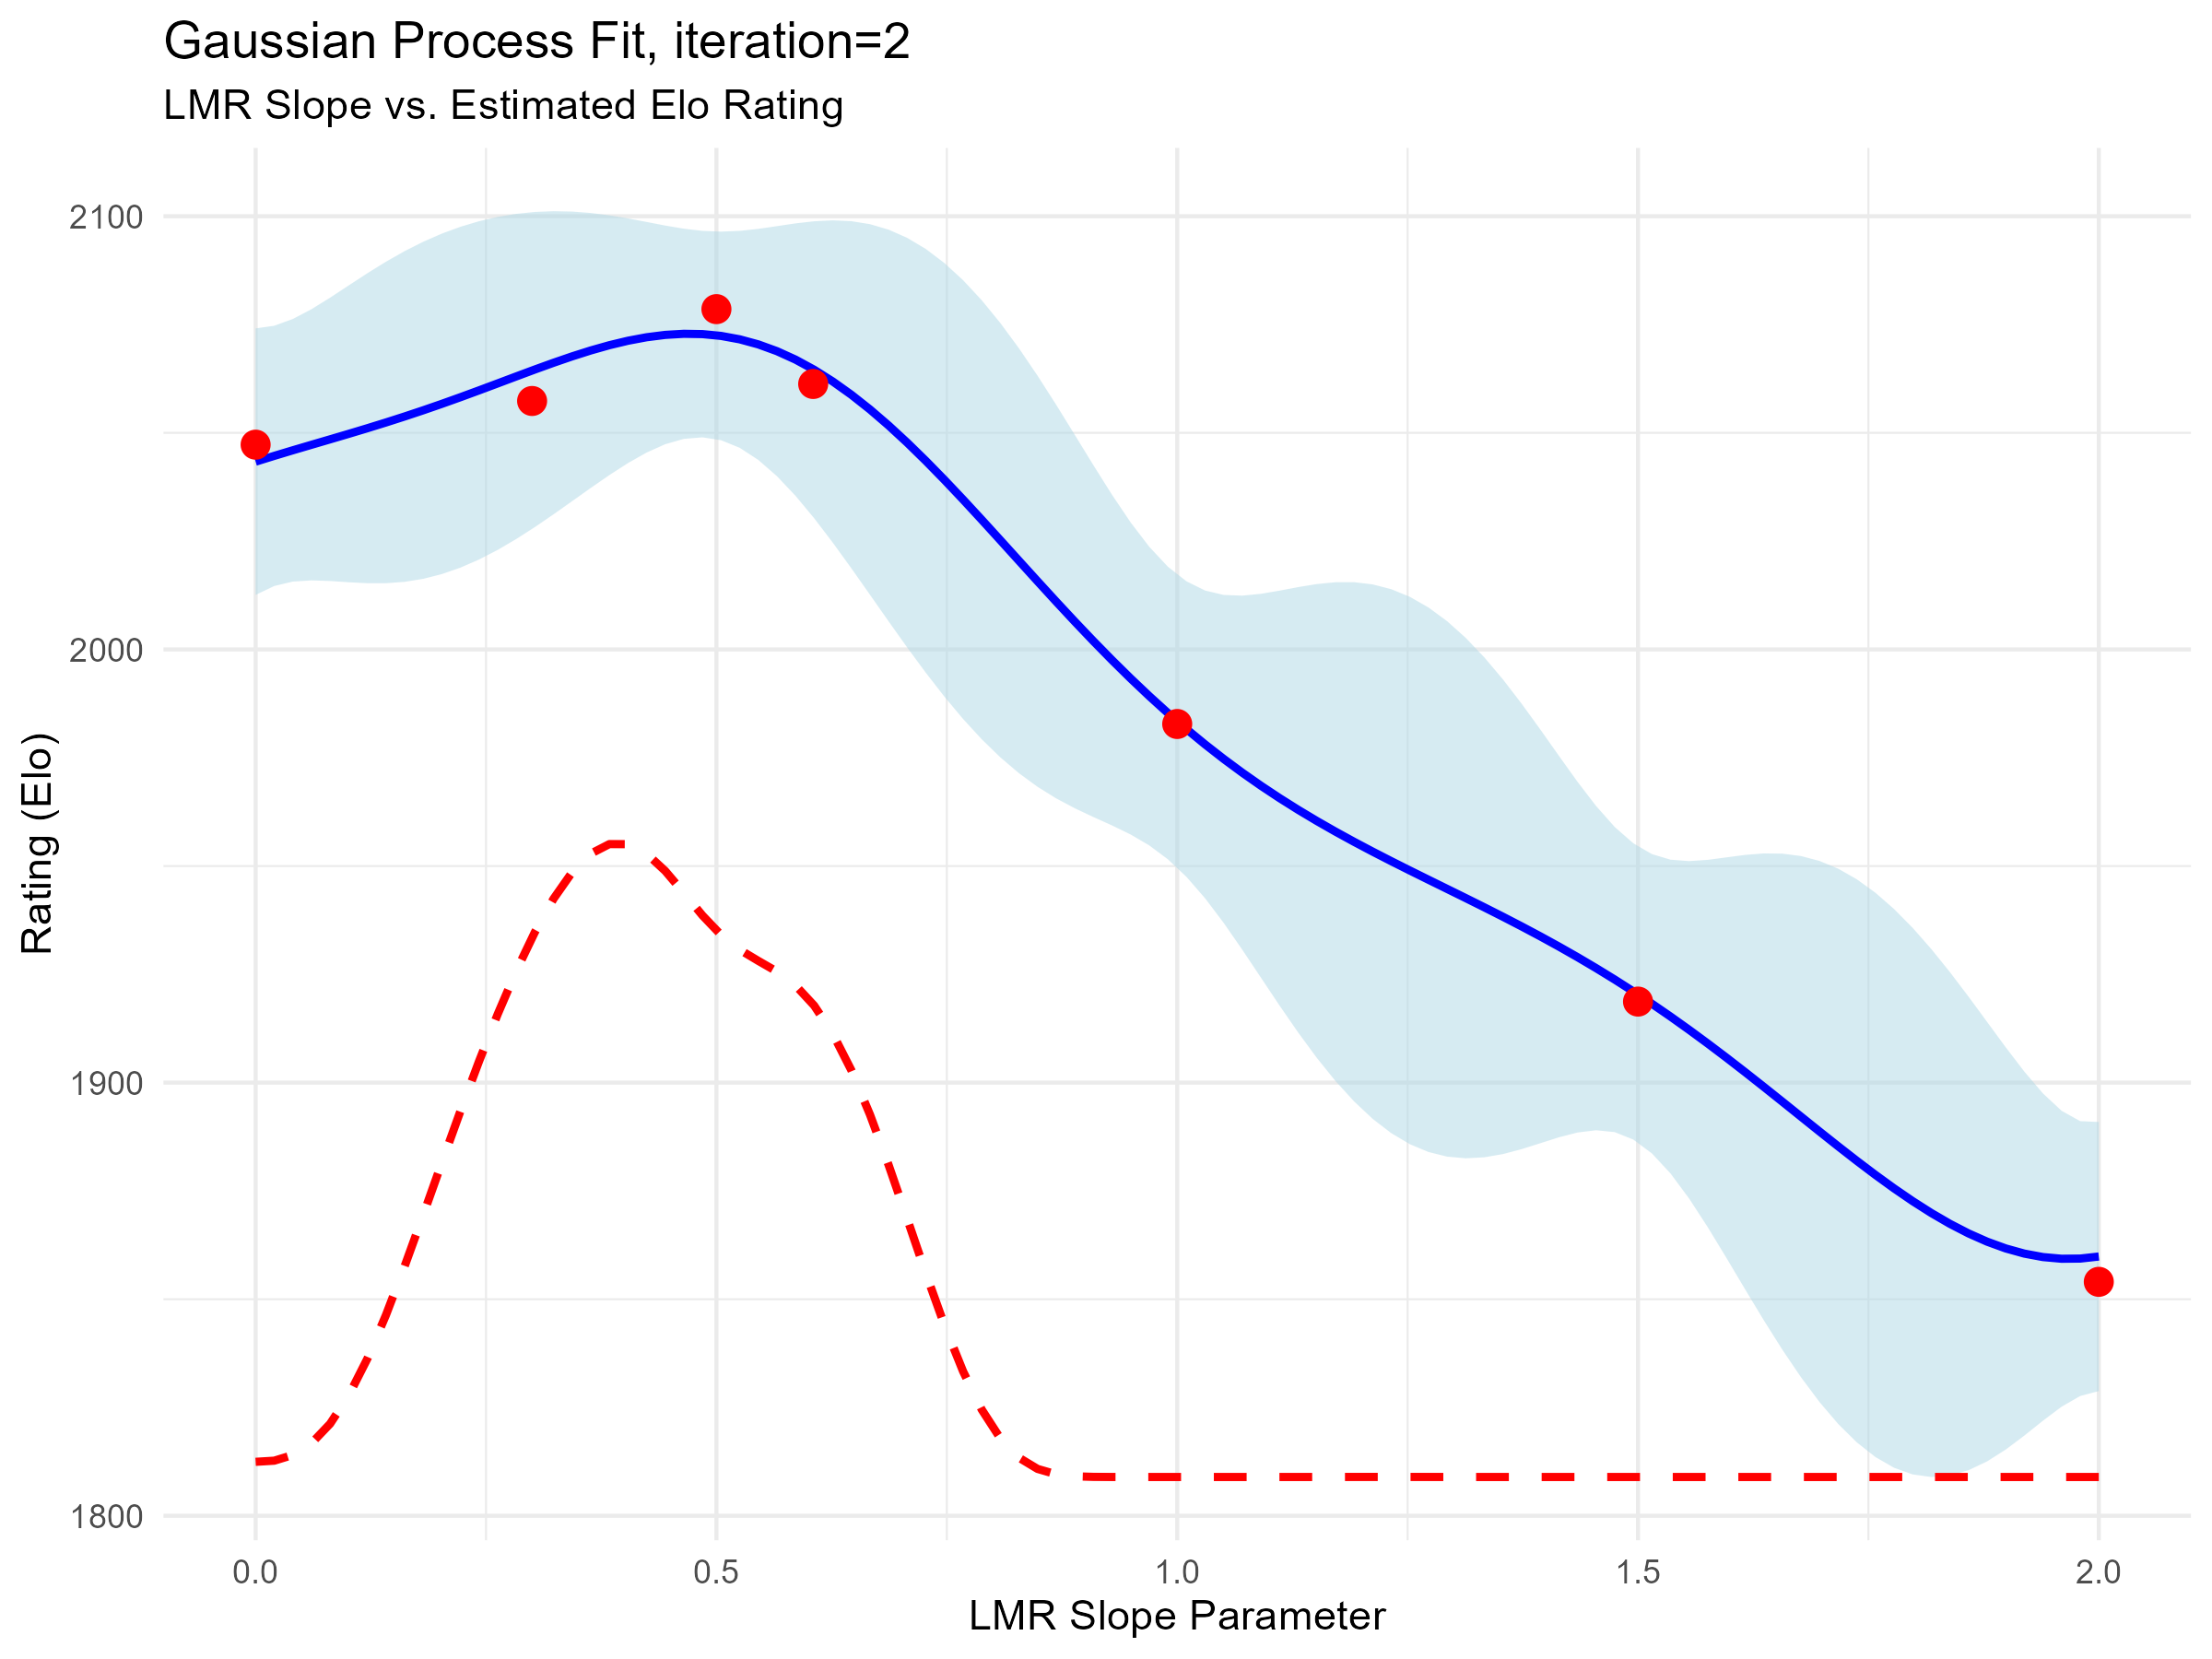
\includegraphics[width=0.8\textwidth]{optimization_iteration_2.png}
    \caption{GP fit after Iteration 2.}
    \label{fig:iter2}
\end{figure}

\begin{figure}[H]
    \centering
    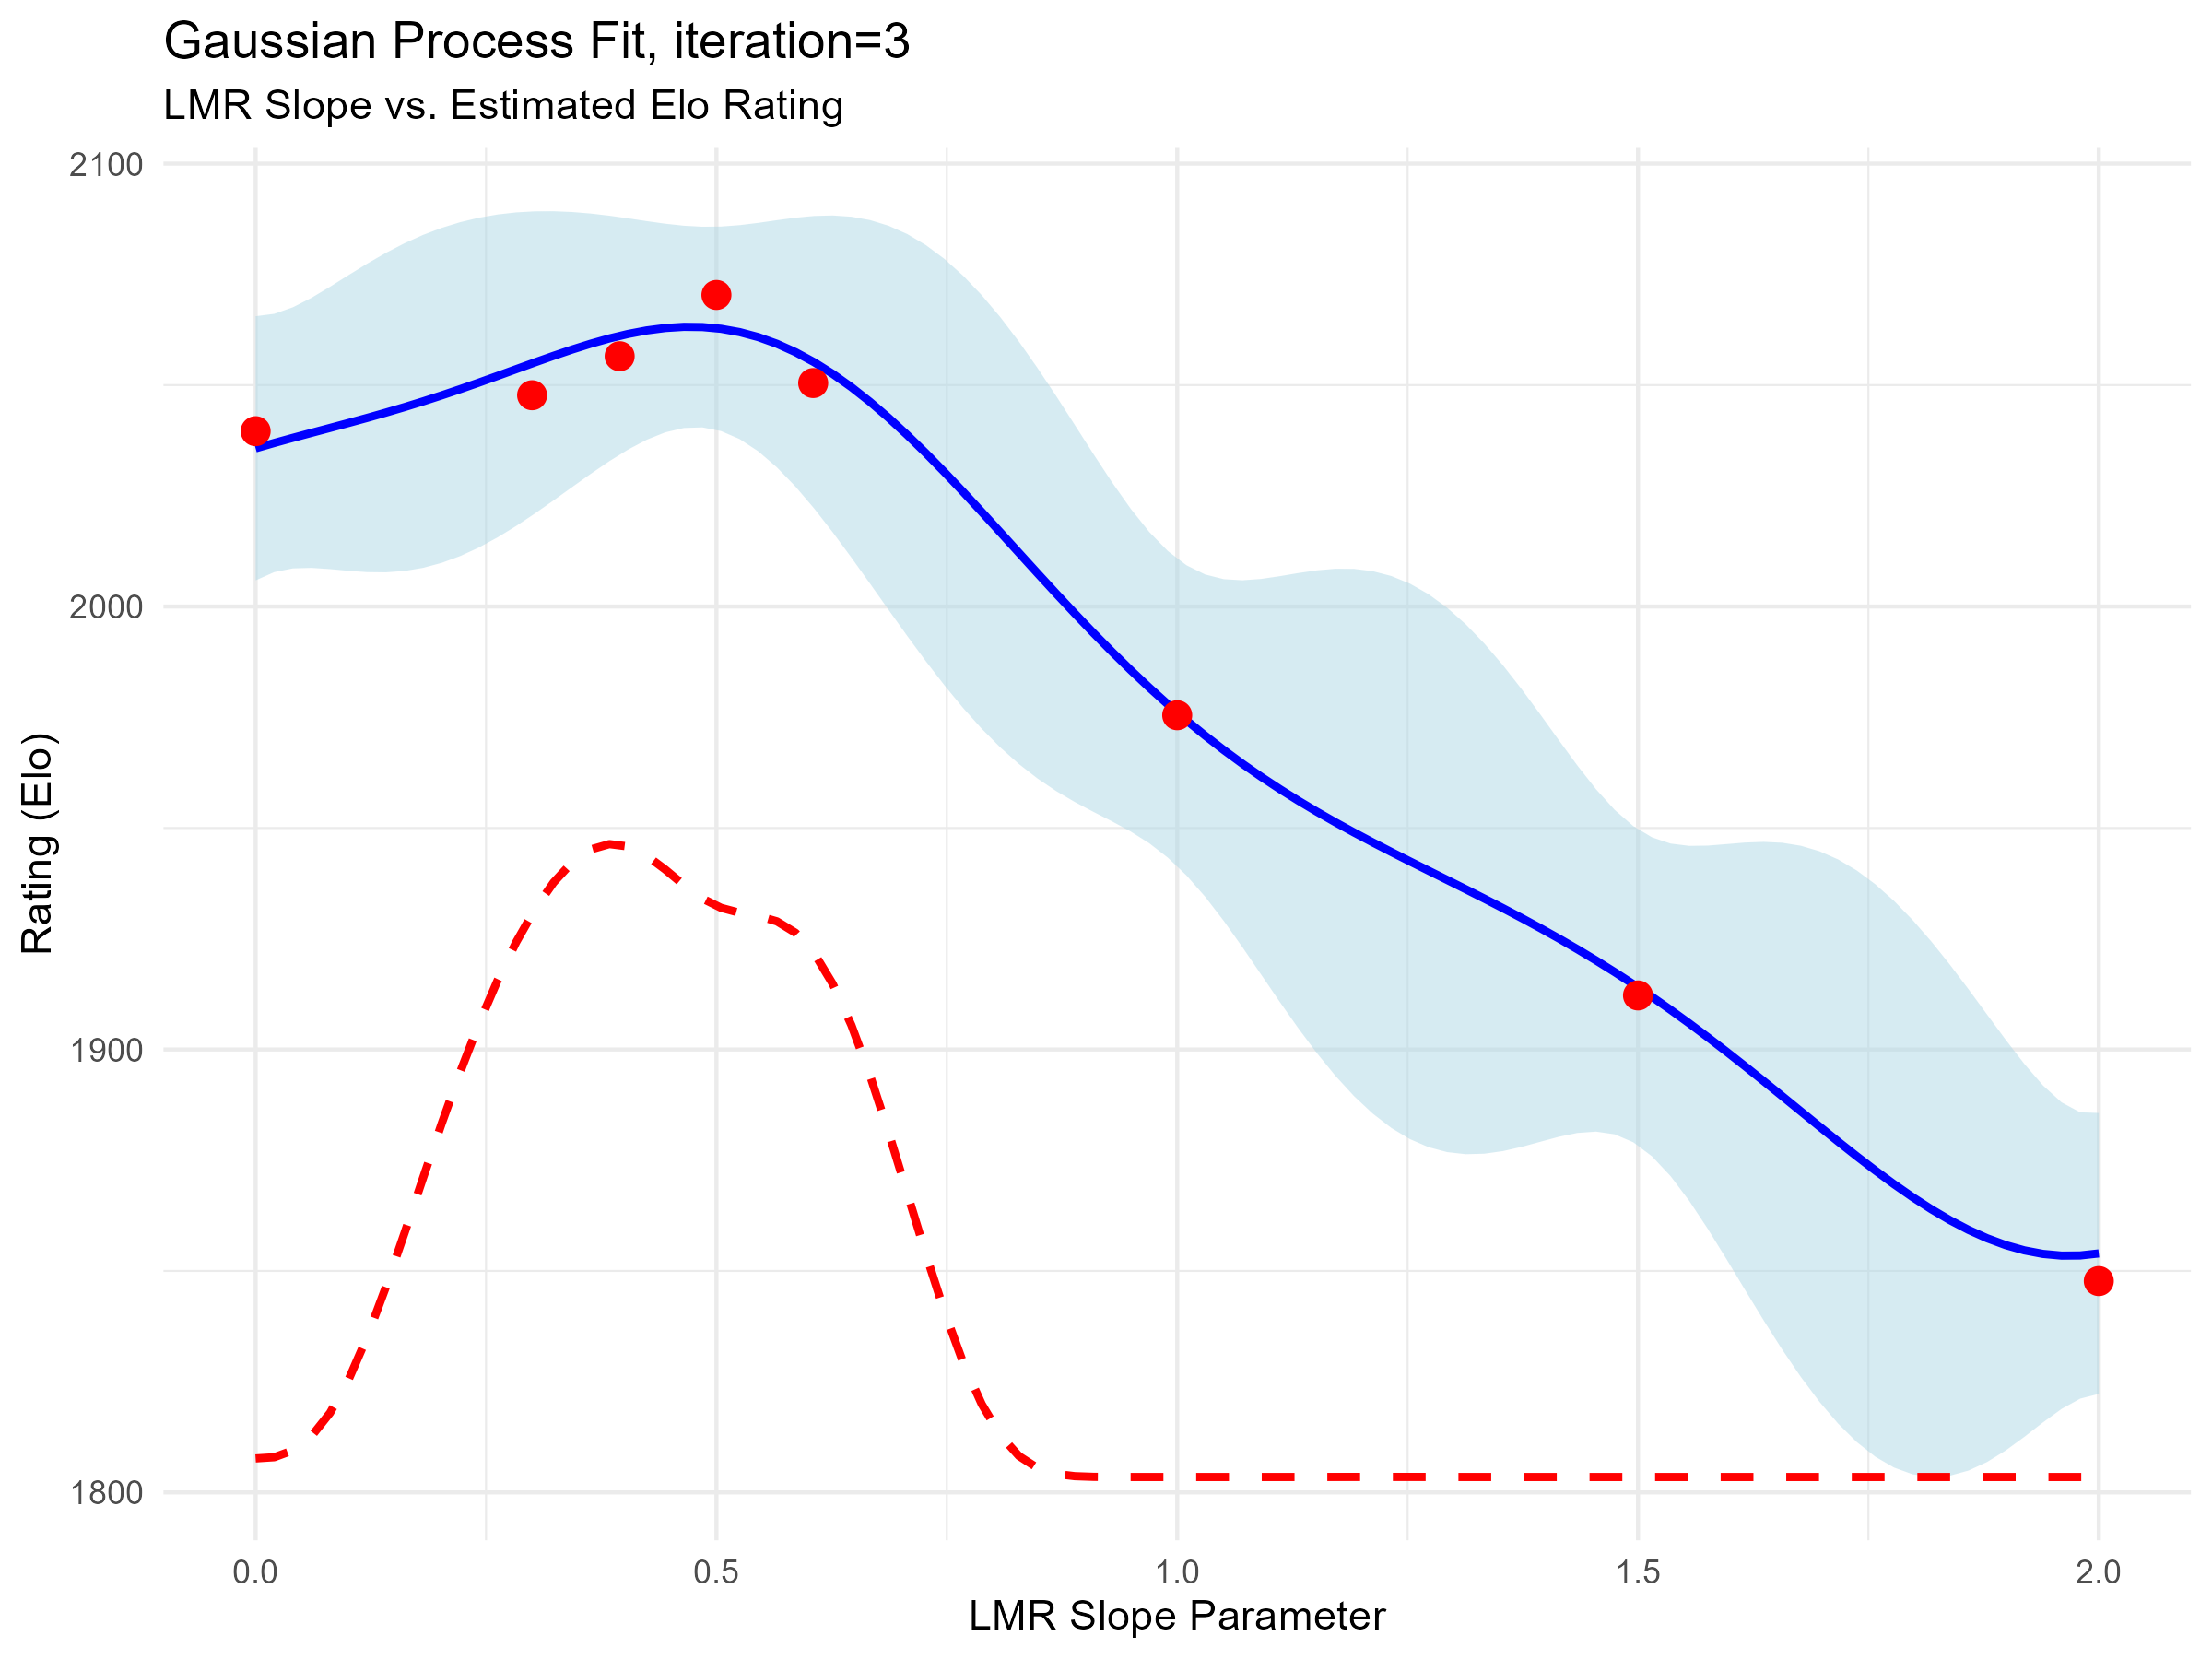
\includegraphics[width=0.8\textwidth]{optimization_iteration_3.png}
    \caption{GP fit after Iteration 3.}
    \label{fig:iter3}
\end{figure}

\begin{figure}[H]
    \centering
    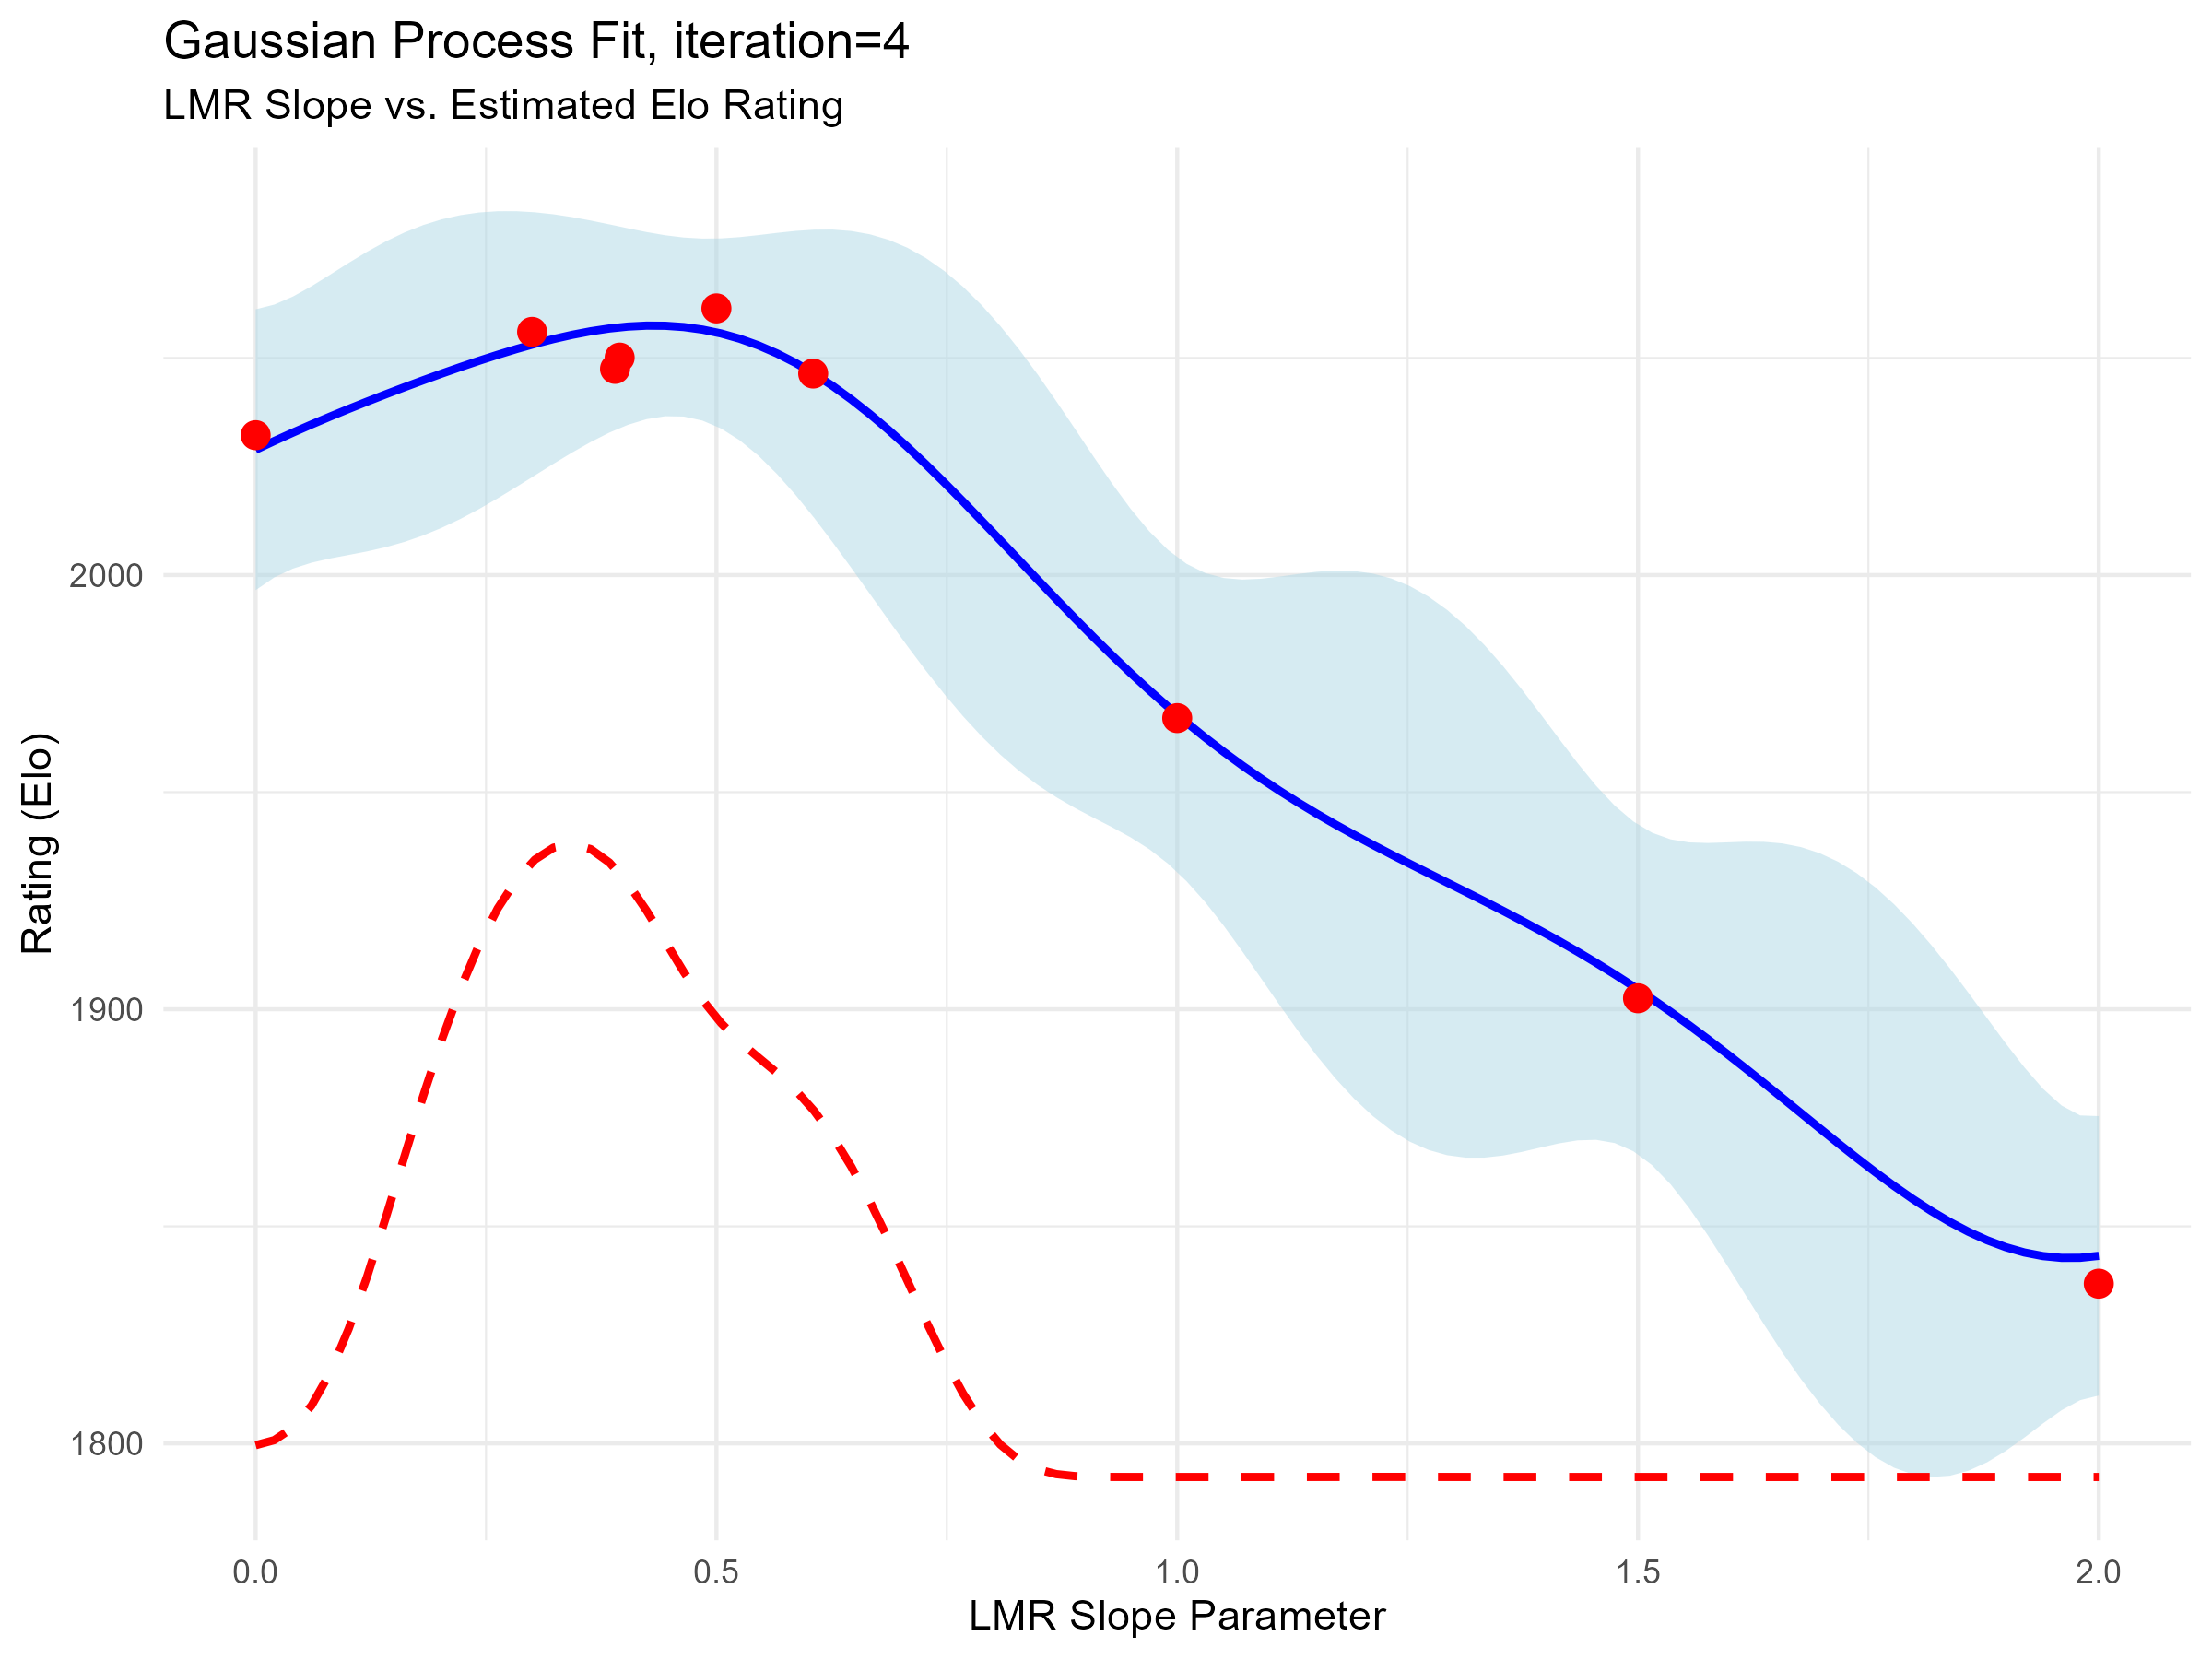
\includegraphics[width=0.8\textwidth]{optimization_iteration_4.png}
    \caption{GP fit after Iteration 4.}
    \label{fig:iter4}
\end{figure}

\begin{figure}[H]
    \centering
    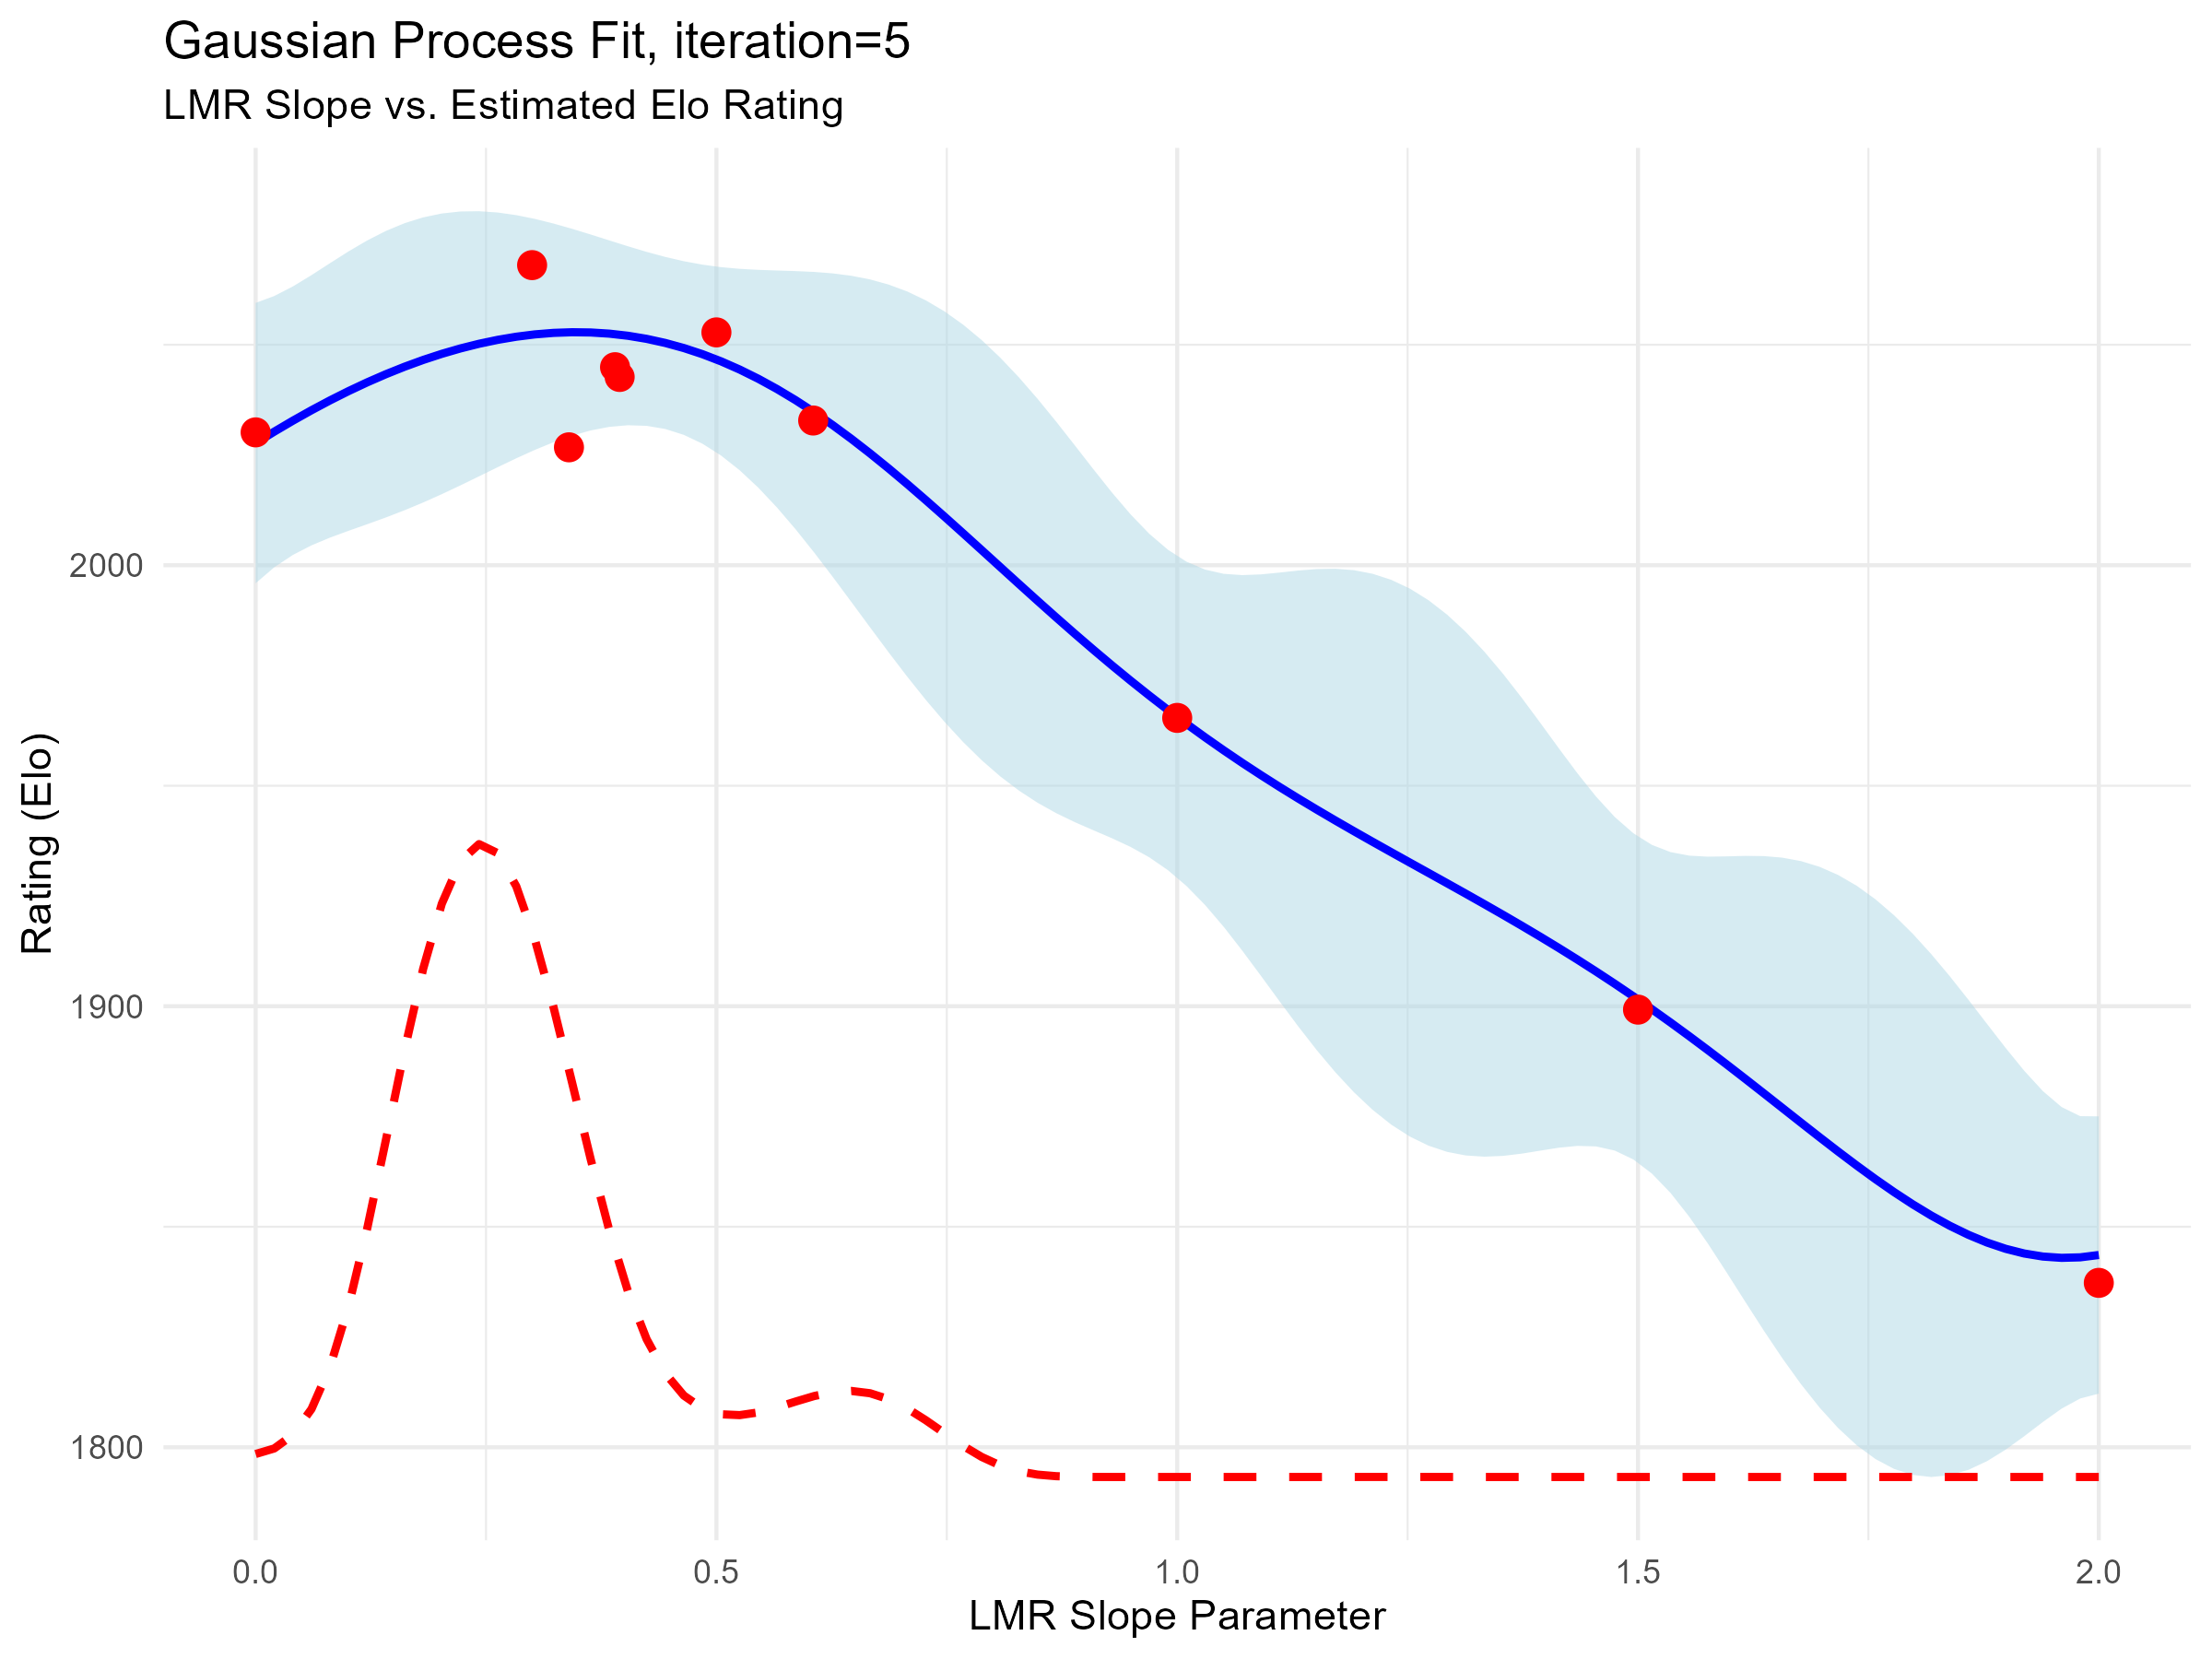
\includegraphics[width=0.8\textwidth]{optimization_iteration_5.png}
    \caption{After testing the new engine 0.34 in Iteration 5 and generating games, the rating model now rates 0.3 higher than the previous maximum of 0.5}
    \label{fig:iter5}
\end{figure}

\begin{figure}[H]
    \centering
    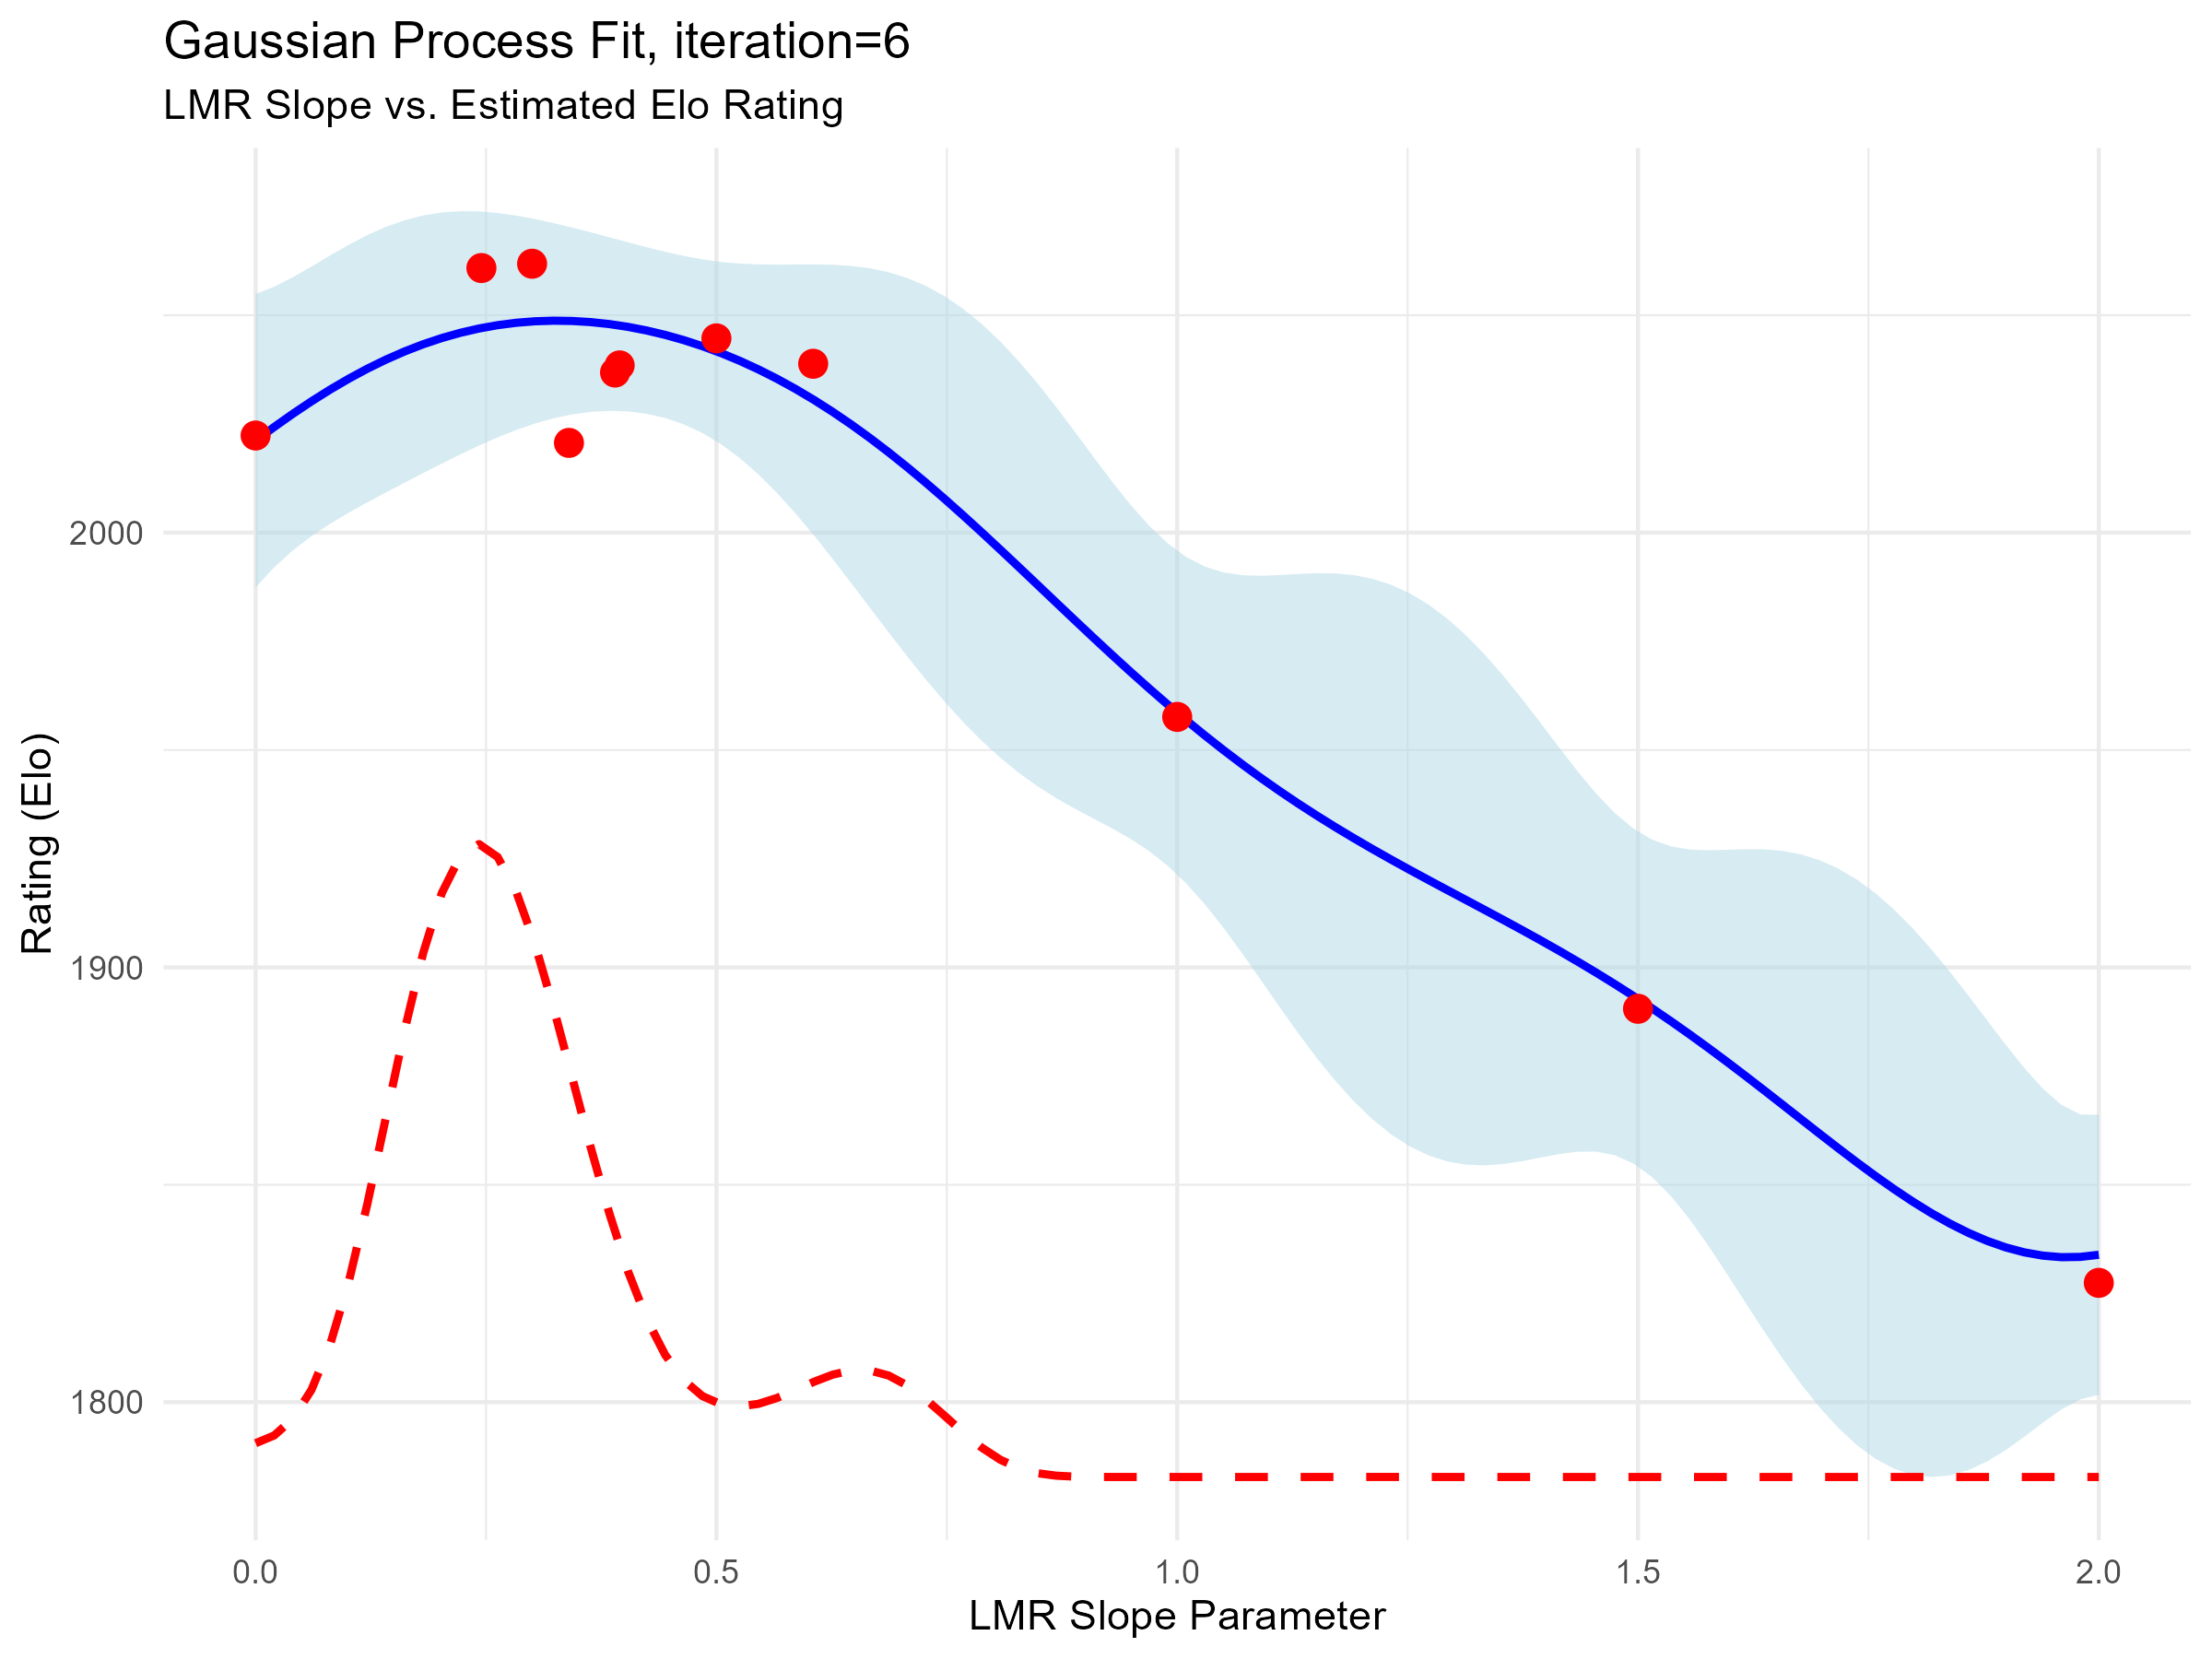
\includegraphics[width=0.8\textwidth]{optimization_iteration_6.png}
    \caption{GP fit after Iteration 6.}
    \label{fig:iter6}
\end{figure}

\begin{figure}[H]
    \centering
    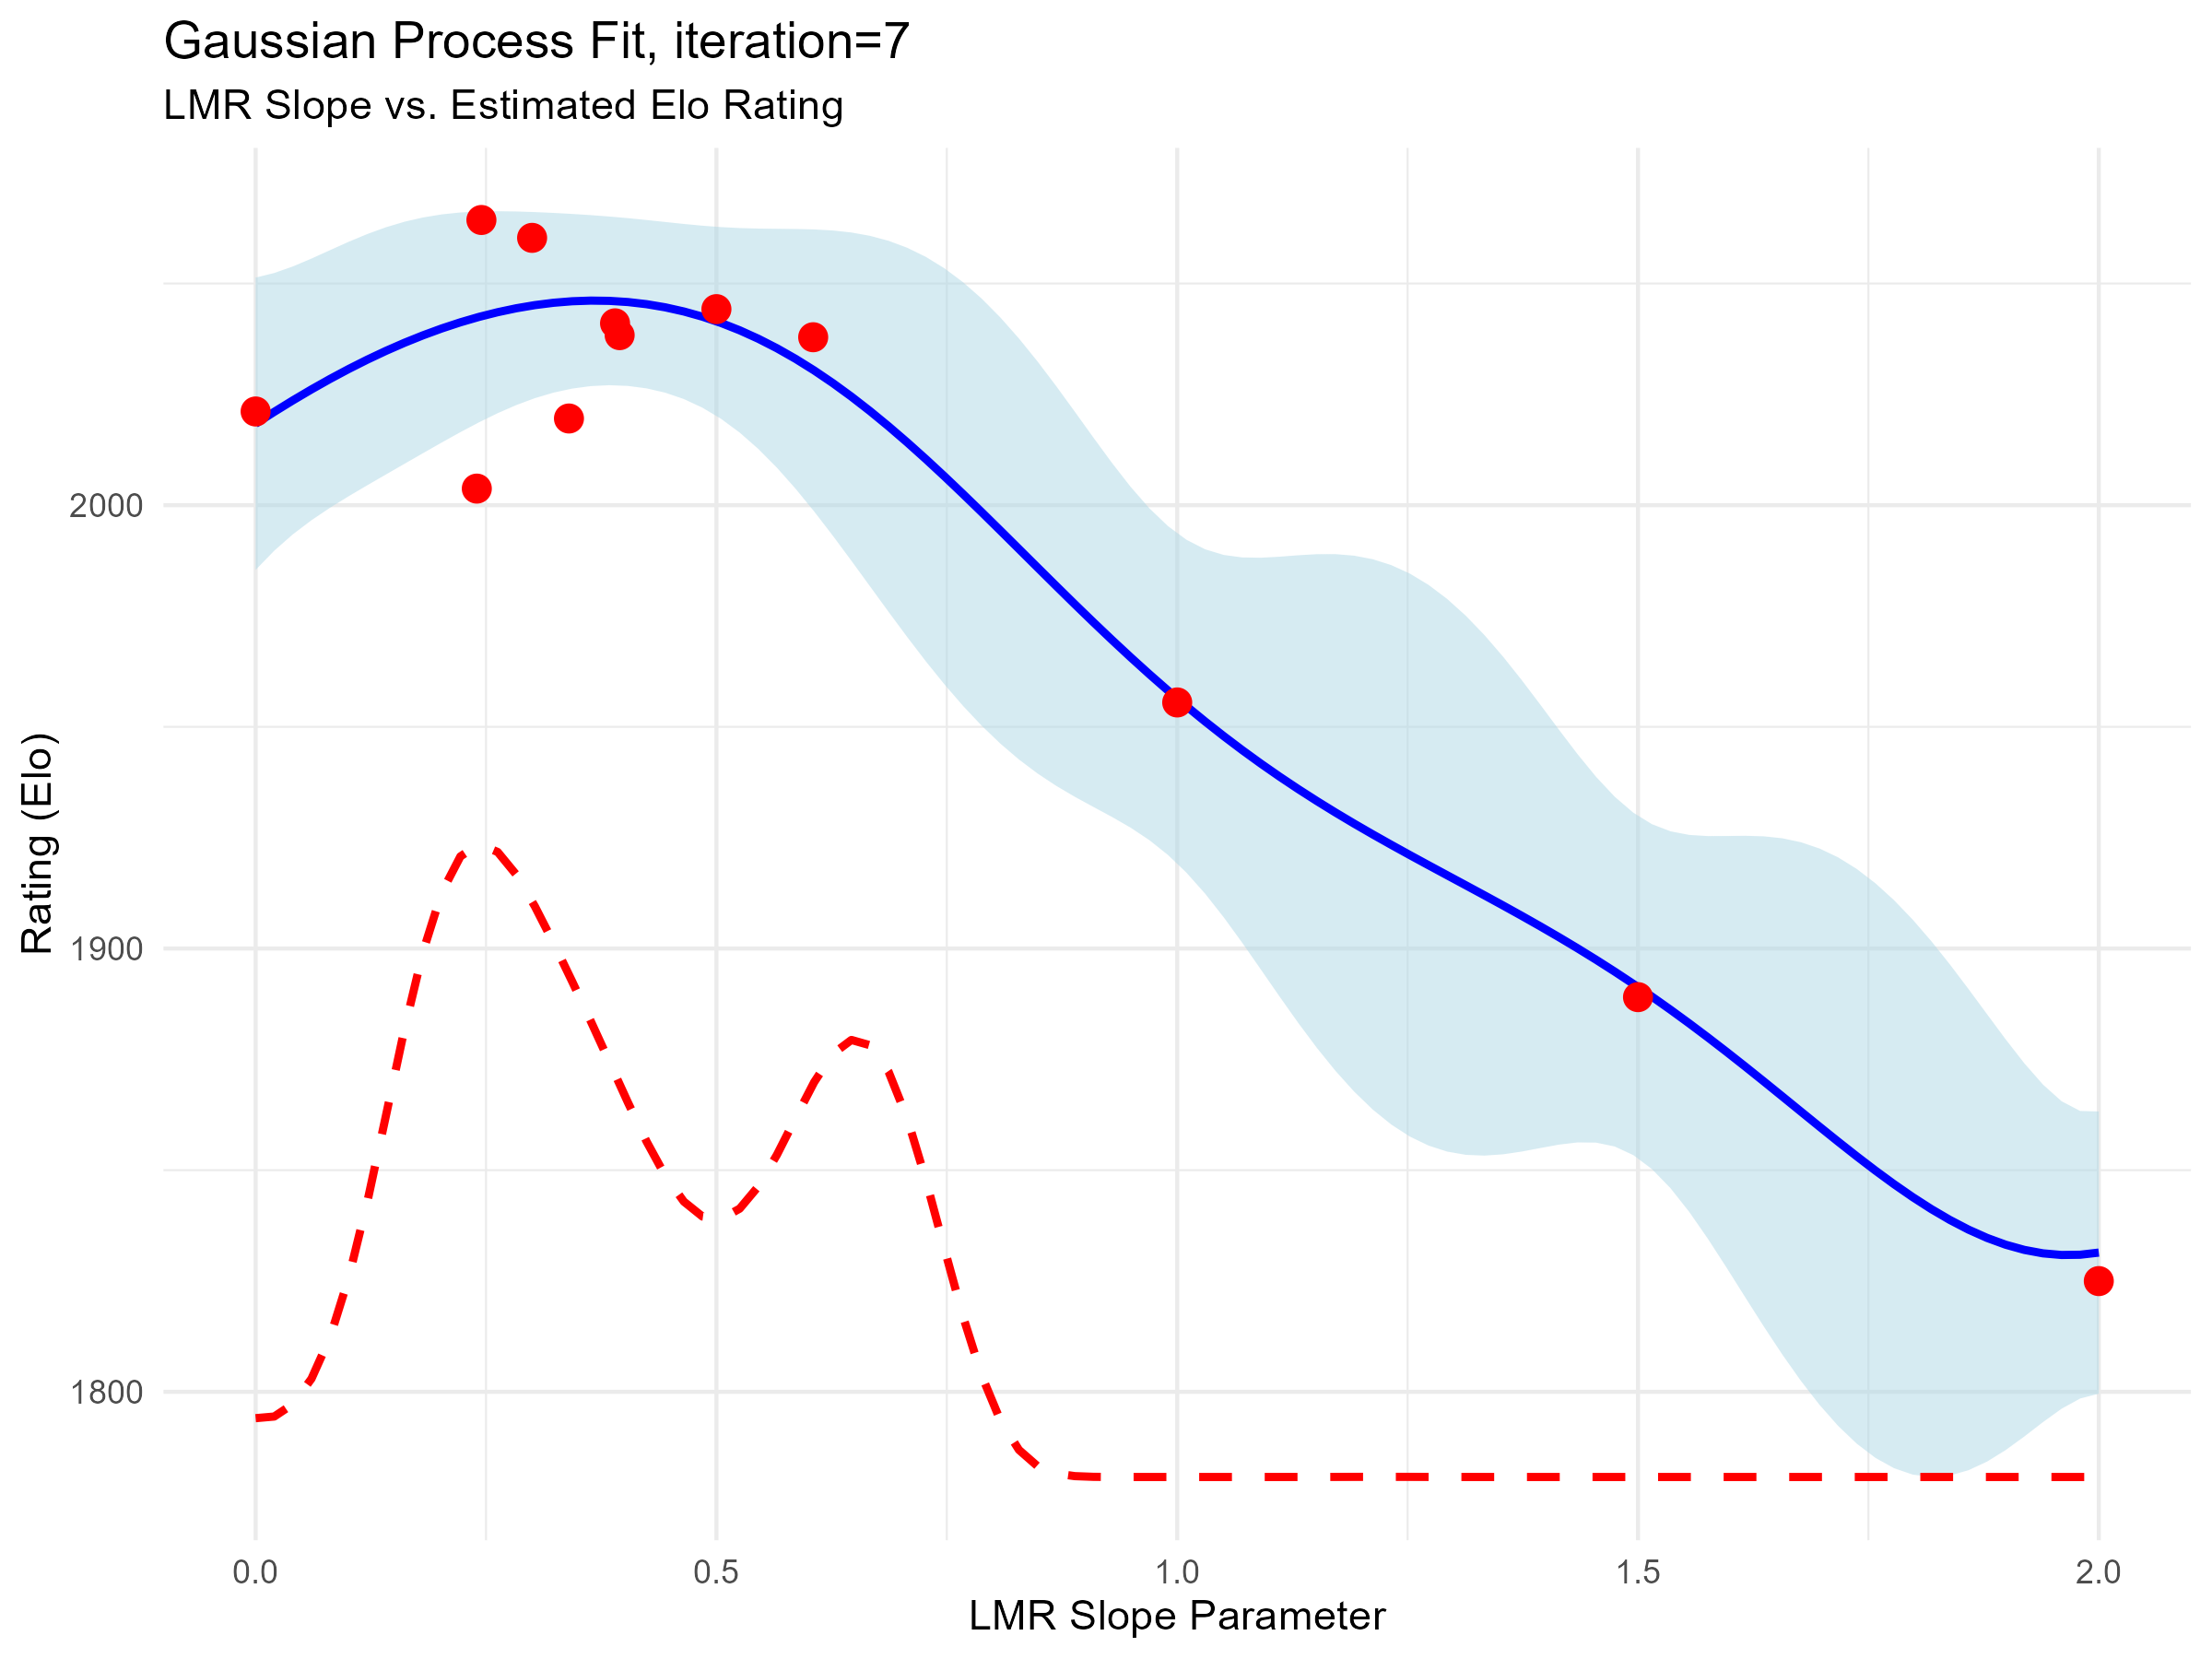
\includegraphics[width=0.8\textwidth]{optimization_iteration_7.png}
    \caption{GP fit after Iteration 7.}
    \label{fig:iter7}
\end{figure}

Our loop terminated during the $8$th iteration with:

\begin{verbatim}
Iteration 8:
Current Best LMR_slope candidate: 0.245 
Proposed New Slope:  0.245
expected improvement:    0.1724
probability of improvement:    0.0360 (3.6\%)
\end{verbatim}

The termination happened, because we specified in the code to terminate if the same value  is tested twice. In hindsight, since there are noisy measurements, it would have made sense to generate more games with the $0.245$ parameter, also in view of the Data after $7$ iterations:

\begin{figure}[H]
    \centering
    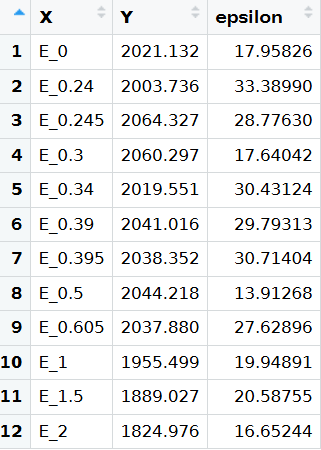
\includegraphics[]{D_after_loop.png}
    \caption{D after Iteration 7.}
    \label{fig:D7}
\end{figure}

There are several parameters with ratings close to another, and still quite some variance. The proposed "best parameter" has positive score in all the mini-matches, except against E\_605:

\begin{figure}[H]
    \centering
    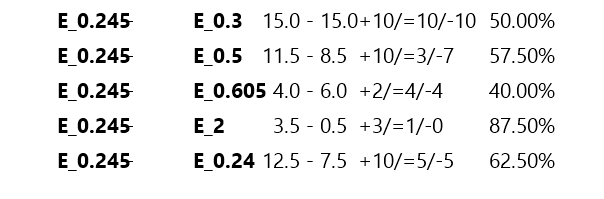
\includegraphics[]{E_0245_results.png}
    \caption{Results of "best" engine}
    \label{fig:E_0245}
\end{figure}


\section{Code}
Attached is the full code from our implementation:
\begin{verbatim}
library(Rschach)
library(dplyr)
library(tidyverse)
library(ggplot2)

# Output filenames
pgn_filename <- "tournament_games.pgn"
csv_filename <- "tournament_results.csv"

# Time control
TC_BASE <- 30   # base time in milliseconds
TC_INC  <- 0 # increment in milliseconds
  #according to the documentation, tc_base and tc_inc are specified in seconds,
  #but after initial run I suspect it must be microseconds --> *1000

# we always play N_POSITIONS different positions, each position 2x (flip colors)
N_POSITIONS <- 25 

#load opening book
opening_book <- read.csv("8moves_v3.epd", header = FALSE)[[1]]

# -----------------------------------
# Step 1: Initialization
# -----------------------------------

# We initialize five engines with LMR_slope parameters {0, 0.5, 1.0, 1.5, 2.0}
# and run a big tournament, where each pair plays N_POSITIONS*2 games

# Values for LMR_slope
param_values <- c(0, 0.5, 1.0, 1.5, 2.0)

# Create engine instances
engines <- vector("list", length(param_values))

for (i in seq_along(param_values)) {
  #note: I originally tried to initalize the engines using a separate function,
  #but weird stuff happened to the engine-objects that were returned...
  #somehow, returning the Engine() objects made some pointers do weird stuff.
  #since I didn't find out what the problem was, I decided to do it "manually"
  current_LMRslope <- param_values[i]
  engine_name   <- paste0("E_", current_LMRslope)
  
  # Define the parameters for this specific engine
  current_params <- list(NMP_intercept = 3,
                         NMP_slope = 0,
                         LMR_intercept = 1,
                         RFP_intercept = -30,
                         RFP_slope = 150,
                         LMR_slope = current_LMRslope)
  e <- Engine(engine_name)
  e$set.params(current_params)
  
  engines[[i]] <- e
}

# Assign names to the list for easy access (e.g., engines$E_1.5)
names(engines) <- paste0("E_", param_values)

#generate N_POSITIONS random starting positions from the opening book
tournament_openings <- opening_book[sample(length(opening_book), N_POSITIONS)]

games <- play.tournament(engines,
                         book = tournament_openings,
                         nr_rounds = 25,
                         repeated = TRUE,
                         tc_base = TC_BASE*1000,
                         tc_inc = TC_INC*1000,
                         verbose = 1)

################
# Create pgn and save results to .csv file
################
pgn(games, file = pgn_filename)

lines <- readLines(pgn_filename)
# Extract fields
whites  <- gsub('\\[White "|"\\]', "", grep('\\[White ".*"\\]', lines, value = TRUE))
blacks  <- gsub('\\[Black "|"\\]', "", grep('\\[Black ".*"\\]', lines, value = TRUE))
results <- gsub('\\[Result "|"\\]', "", grep('\\[Result ".*"\\]', lines, value = TRUE))
tc_val <- paste0(TC_BASE, "+", TC_INC)
time_controls <- rep(tc_val, length(results))
# Create dataframe with columns: white, black, result, timecontrol
results_df <- data.frame(
  white = whites, 
  black = blacks, 
  result = results, 
  timecontrol = time_controls, 
  stringsAsFactors = FALSE
)
write.csv(results_df, csv_filename, row.names = FALSE, quote = FALSE)

#tournament results (table generated with chessbase)
#     1	       2	           3	           4	           5	
# 1	E_0.5	27.0 - 23.0   31.0 - 19.0   38.5 - 11.5   39.0 - 11.0 **					135.5/200
# 2	E_0	  23.0 - 27.0   30.5 - 19.5   35.0 - 15.0   40.0 - 10.0	  **				128.5/200
# 3	E_1	  19.0 - 31.0   19.5 - 30.5   26.0 - 24.0   37.0 - 13.0		  **			101.5/200
# 4	E_1.5	11.5 - 38.5   15.0 - 35.0   24.0 - 26.0   28.0 - 22.0			  **		78.5/200
# 5	E_2	  11.0 - 39.0   10.0 - 40.0   13.0 - 37.0   22.0 - 28.0				  **	56.0/200

#current "best engine" beats the current weakest engine approximately 4-1,
#which suggests a rating difference of ~240 elo points.
#--> for rating modelling, we could choose the prior to have
#    standard deviation e.g. 150, but 200 as in Task 1 should also be fine


# -----------------------------------
# Step 2: Initial Modelling
# -----------------------------------

#We first run the rating model from task 1 on the tournament results,
#obtaining data X = {0, 0.5, 1.0, 1.5, 2.0}, Y = {\mu(E_0), \mu(E_0.5), ..., \mu(E_2)}
#with noise \epsilon = {sd(E_0), sd(E_0.5), ..., sd(E_2)} (sd = standard deviation)

#load and compile stan model from part 1
library(rstan)
options(mc.cores = parallel::detectCores())
rstan_options(auto_write = TRUE)
stanmodel <- stan_model("elo_model.stan") #slightly modified model from task 1
source("../src/preprocessing.R")

#returns dataframe with columns X (=engine names), Y (=mean rating), epsilon (=sd)
run_elo_model <- function(results_csv, stan_model){

  # ...(code from task 1, slightly modified)

  games <- read_csv(results_csv, show_col_types = FALSE)
  engine_names <- sort(get_players(results_csv))
  n_engines <- length(engine_names)
  engine_to_idx <- setNames(1:n_engines, engine_names)
  games <- games %>%
    mutate(
      white_score = case_when(
        result == "1-0" ~ 1.0,
        result == "1/2-1/2" ~ 0.5,
        result == "0-1" ~ 0.0
      ),
      white_idx = engine_to_idx[white],
      black_idx = engine_to_idx[black]
    )
  stan_data <- list(
    N = nrow(games),
    K = n_engines,
    white = games$white_idx,
    black = games$black_idx,
    score = games$white_score
  )
  cat("Running MCMC sampling...\n")
  fit <- sampling(
    stan_model,
    data = stan_data,
    chains = 4,
    iter = 2000,
    warmup = 1000,
    control = list(adapt_delta = 0.95)
  )
  
  #Use rstan::extract to avoid conflict with tidyr
  rating_samples <- rstan::extract(fit, pars = "rating_absolute")$rating_absolute
  rating_summary <- data.frame(
    X = engine_names,
    Y = colMeans(rating_samples),
    epsilon = apply(rating_samples, 2, sd)
  )
  
  return(rating_summary)
}
}

D <- run_elo_model("tournament_results.csv", stanmodel)

#we need functionality to generate a GP with "known" noise
#the library GauPro doesn't support this as far as I found out,
#but the following library has built-in functions for this:
#install.packages("DiceKriging")
library(DiceKriging)
kernel_type <- "gauss"

# Fit the GP
gp_model <- km(
  design = data.frame(x = as.numeric(sub("E_", "", D$X))), 
  response = D$Y, 
  covtype = kernel_type, 
  noise.var = D$epsilon^2,
  upper = 0.3 #upper bound for length-scale parameter
)

calculate_expected_improvement <- function(pred, y_best){
  #pred = prediction of GP model for some points X
  #returns expected improvement for points X
  
  mu <- pred$mean
  sigma <- pred$sd
  sigma <- pmax(sigma, 1e-9) # avoid division by zero

  # Calculate Expected Improvement
  Z <- (mu - y_best) / sigma
  # Formula: (mu - y_best) * Phi(Z) + sigma * phi(Z)
  ei <- (mu - y_best) * pnorm(Z) + sigma * dnorm(Z)
  
  return(ei)
}

plot_gaussian_process <- function(gp, D, x_grid, plot_output_name, iteration){
  # Predict GP values for sequence of points x_grid
  pred <- predict(object=gp,
                  newdata=x_grid,
                  type = "UK") #type=universal kriging -> uncertainty in means
  
  # Calculate 95% Confidence Intervals
  lower_bound <- pred$mean - 1.96 * pred$sd
  upper_bound <- pred$mean + 1.96 * pred$sd
  
  # Calculate Expected Improvement for the same grid
  ei_values <- calculate_expected_improvement(pred, max(D$Y))
  # EI values are small (e.g., 0-10), while Ratings are large (e.g., 2000).
  # We scale EI up to fit visually on the plot.
  ylim_primary <- range(c(lower_bound, upper_bound, D$Y))
  plot_height  <- diff(ylim_primary)
  max_ei       <- max(ei_values)
  # Prevent scaling error if max_ei is 0
  if(max_ei == 0) max_ei <- 1 
  # Scale factor: stretches EI to occupy roughly 20% of the plot height
  scale_factor <- (plot_height * 0.5) / max_ei 
  # Shift factor: moves the EI line to the bottom of the rating graph
  shift_factor <- min(lower_bound)
  
  # Combine all data into a dataframe for plotting
  plot_data <- data.frame(
    x = x_grid,
    y = pred$mean,
    lower = lower_bound,
    upper = upper_bound,
    ei_scaled = (ei_values * scale_factor) + shift_factor
  )
  
  # Original data points for reference
  original_points <- data.frame(x = as.numeric(sub("E_", "", D$X)), y=D$Y)
  
  gp_plot <- ggplot(plot_data, aes(x = x, y = y)) +
    # 1. Add the shaded confidence interval (95%)
    geom_ribbon(aes(ymin = lower, ymax = upper), fill = "lightblue", alpha = 0.5) +
    
    # 2. Add the GP mean prediction line
    geom_line(color = "blue", linewidth = 1) +
    
    # 3. Add the original observed data points (Red dots)
    geom_point(data = original_points, aes(x = x, y = y), color = "red", size = 3) +
    
    # 4. Expected Improvement
    geom_line(aes(y = ei_scaled), color = "red", linewidth = 1, linetype = "dashed") +
    
    # Styling
    labs(title = paste0("Gaussian Process Fit, iteration=", iteration),
         subtitle = "LMR Slope vs. Estimated Elo Rating",
         x = "LMR Slope Parameter",
         y = "Rating (Elo)") +
    theme_minimal()
  
   ggsave(filename = paste0(plot_output_name, ".png"), 
         plot = gp_plot, 
         width = 8, 
         height = 6, 
         dpi = 300)
}

x_grid <- data.frame(x=seq(0, 2, length.out = 100))
plot_gaussian_process(gp_model, D, x_grid, "initial_plot", 0)


# -----------------------------------
# Step 3: Optimization loop
# -----------------------------------

iteration <- 1

x_grid_search <- seq(0, 2.0, by = 0.005)

while(TRUE){
  cat(paste0("\nIteration ", iteration, ":\n"))
  
  y_best <- max(D$Y)
  # Find the LMRslope with maximum Y (=rating)
  best_engine_row <- D[which.max(D$Y), ]
  best_slope <- as.numeric(sub("E_", "", best_engine_row$X))
  
  # predict on search grid
  pred_grid <- predict(gp_model, newdata = data.frame(x = x_grid_search), type = "UK")
  
  # calculate Expected Improvement
  expected_improvement_values <- calculate_expected_improvement(pred_grid, y_best)
  
  # calculate Probability of Improvement
  sigma <- pmax(pred_grid$sd, 1e-9) #avoid dividing by 0
  Z <- (pred_grid$mean - y_best) / sigma
  probability_of_improvement_values <- pnorm(Z)

  # Find best candidate
  best_idx <- which.max(expected_improvement_values)
  best_x <- x_grid_search[best_idx]
  max_ei <- expected_improvement_values[best_idx]
  max_pi <- probability_of_improvement_values[best_idx]
  
  # User Interaction
  cat(sprintf("Current Best LMR_slope candidate: %.2f \n", best_slope))
  cat(sprintf("Proposed New Slope:  %.2f\n", best_x))
  cat(sprintf("expected improvement:    %.4f\n", max_ei))
  cat(sprintf("probability of improvement:    %.4f (%.1f%%)\n", max_pi, max_pi*100))
  # Check thresholds
  if (max_pi < 0.01) {
    cat("(!) Probability of improvement is low (<1%).\n")
  }
  
  user_input <- readline(prompt = "Proceed? (y/n): ")
  if (tolower(user_input) != "y") {
    cat("Optimization stopped by user.\n")
    break
  }
  
  #check if new slope already exists (or is numerically very close to an existing one)
  if (any(abs(as.numeric(sub("E_", "", D$X)) - best_x) < 1e-4)) {
    cat(sprintf("Slope %.2f already exists - stopping!\n", best_x))
    break
  }
  
  #pick a diverse subset of the previous LMRslope parameters: the two best engines,
   #the median engine and the worst engine
  D_sorted <- D[order(D$Y, decreasing = TRUE), ]
  n_engines <- nrow(D_sorted)
  # Identify the LMR_slope of the engines we want
  best <- as.numeric(sub("E_", "",D_sorted$X[1])) #best engine
  second_best<- as.numeric(sub("E_", "",D_sorted$X[2])) #second best engine
  median <- as.numeric(sub("E_", "",D_sorted$X[ceiling(n_engines / 2)])) #median engine
  worst <- as.numeric(sub("E_", "",D_sorted$X[n_engines])) #worst engine
  
  cat(sprintf("Picked subset: Best=%.2f, 2nd Best=%.2f, Median=%.2f, Worst=%.2f\n", 
              best, second_best, median, worst))
  
  # Initialize New Engine
  new_engine_name <- paste0("E_", best_x)
  new_params <- list(NMP_intercept = 3, 
                     NMP_slope = 0, 
                     LMR_intercept = 1,
                     RFP_intercept = -30, 
                     RFP_slope = 150, 
                     LMR_slope = best_x)
  new_engine <- Engine(new_engine_name)
  new_engine$set.params(new_params)
  
  ###########
  #play games
  ###########
  opponents <- c(best, second_best, median, worst)
  rounds_schedule <- c(15, 10, 5, 2)
  # Loop through the subset indices (up to 4)
  for (i in seq_along(opponents)) {
    opponent_slope <- opponents[i]
    n_rounds <- rounds_schedule[i]
    
    cat(sprintf("  Vs %s: %d rounds... ", opponent_slope, n_rounds))

    # 2. Initialize Opponent Engine
    opponent_engine <- Engine(paste0("E_", opponent_slope))
    opponent_engine$set.params(list(
      NMP_intercept = 3, NMP_slope = 0, LMR_intercept = 1,
      RFP_intercept = -30, RFP_slope = 150, LMR_slope = opponent_slope
    ))
    
    # generate random opening positions
    current_openings <- opening_book[sample(length(opening_book), n_rounds)]
    
    #play match
    match_games <- play.tournament(
      new_engine,
      opponent_engine,
      book = current_openings,
      nr_rounds = n_rounds,
      repeated = TRUE,
      tc_base = TC_BASE * 1000,
      tc_inc = TC_INC * 1000,
      verbose = 1
    )
    
    # Append games to pgn
    temp_pgn <- "temp_match_games.pgn"
    pgn(match_games, file = temp_pgn)
    file.append(pgn_filename, temp_pgn)
    unlink(temp_pgn)
  }
  
  #update .csv
  ############
  lines <- readLines(pgn_filename)
  # Extract fields
  whites  <- gsub('\\[White "|"\\]', "", grep('\\[White ".*"\\]', lines, value = TRUE))
  blacks  <- gsub('\\[Black "|"\\]', "", grep('\\[Black ".*"\\]', lines, value = TRUE))
  results <- gsub('\\[Result "|"\\]', "", grep('\\[Result ".*"\\]', lines, value = TRUE))
  tc_val <- paste0(TC_BASE, "+", TC_INC)
  time_controls <- rep(tc_val, length(results))
  # Create dataframe with columns: white, black, result, timecontrol
  results_df <- data.frame(
    white = whites, 
    black = blacks, 
    result = results, 
    timecontrol = time_controls, 
    stringsAsFactors = FALSE
  )
  write.csv(results_df, csv_filename, row.names = FALSE, quote = FALSE)
  
  # Re-run Elo Model
  ##################
  
  cat("Updating Elo Model ...\n")
  D <- run_elo_model(csv_filename, stanmodel)
  
  # Update Gaussian Process and plotting
  #########################
  cat("Updating Gaussian Process...\n")
  gp_model <- km(
    design = data.frame(x = as.numeric(sub("E_", "", D$X))), 
    response = D$Y, 
    covtype = kernel_type, 
    noise.var = D$epsilon^2,
    upper = 0.3
  )
  plot_filename <- paste0("optimization_iteration_", iteration)
  grid_for_plot <- data.frame(x=seq(0, 2, length.out = 100))
  plot_gaussian_process(gp_model, D, grid_for_plot, plot_filename, iteration)
  
  iteration <- iteration + 1
}
\end{verbatim}
\end{document}